\documentclass[a4paper, oneside]{memoir}
\usepackage[english]{babel}
\usepackage{sheaves}

\makeindex

% 4f6654 green 364f76  blue
\definecolor{titlepagebackground}{HTML}{364f76}
\definecolor{wheat}{HTML}{fcbd53}

% \usepackage{quiver}
\begin{document}

\begin{titlingpage}
\thispagestyle{empty}
\begin{tikzpicture}[remember picture,overlay]
  % dimensions of goncharova-harvesting.jpg: width = 1800 px, height = 1743 px
  \node[xshift=-.5*1800/1743*1.1\paperheight, yshift=-.05\paperheight] at (current page.east) {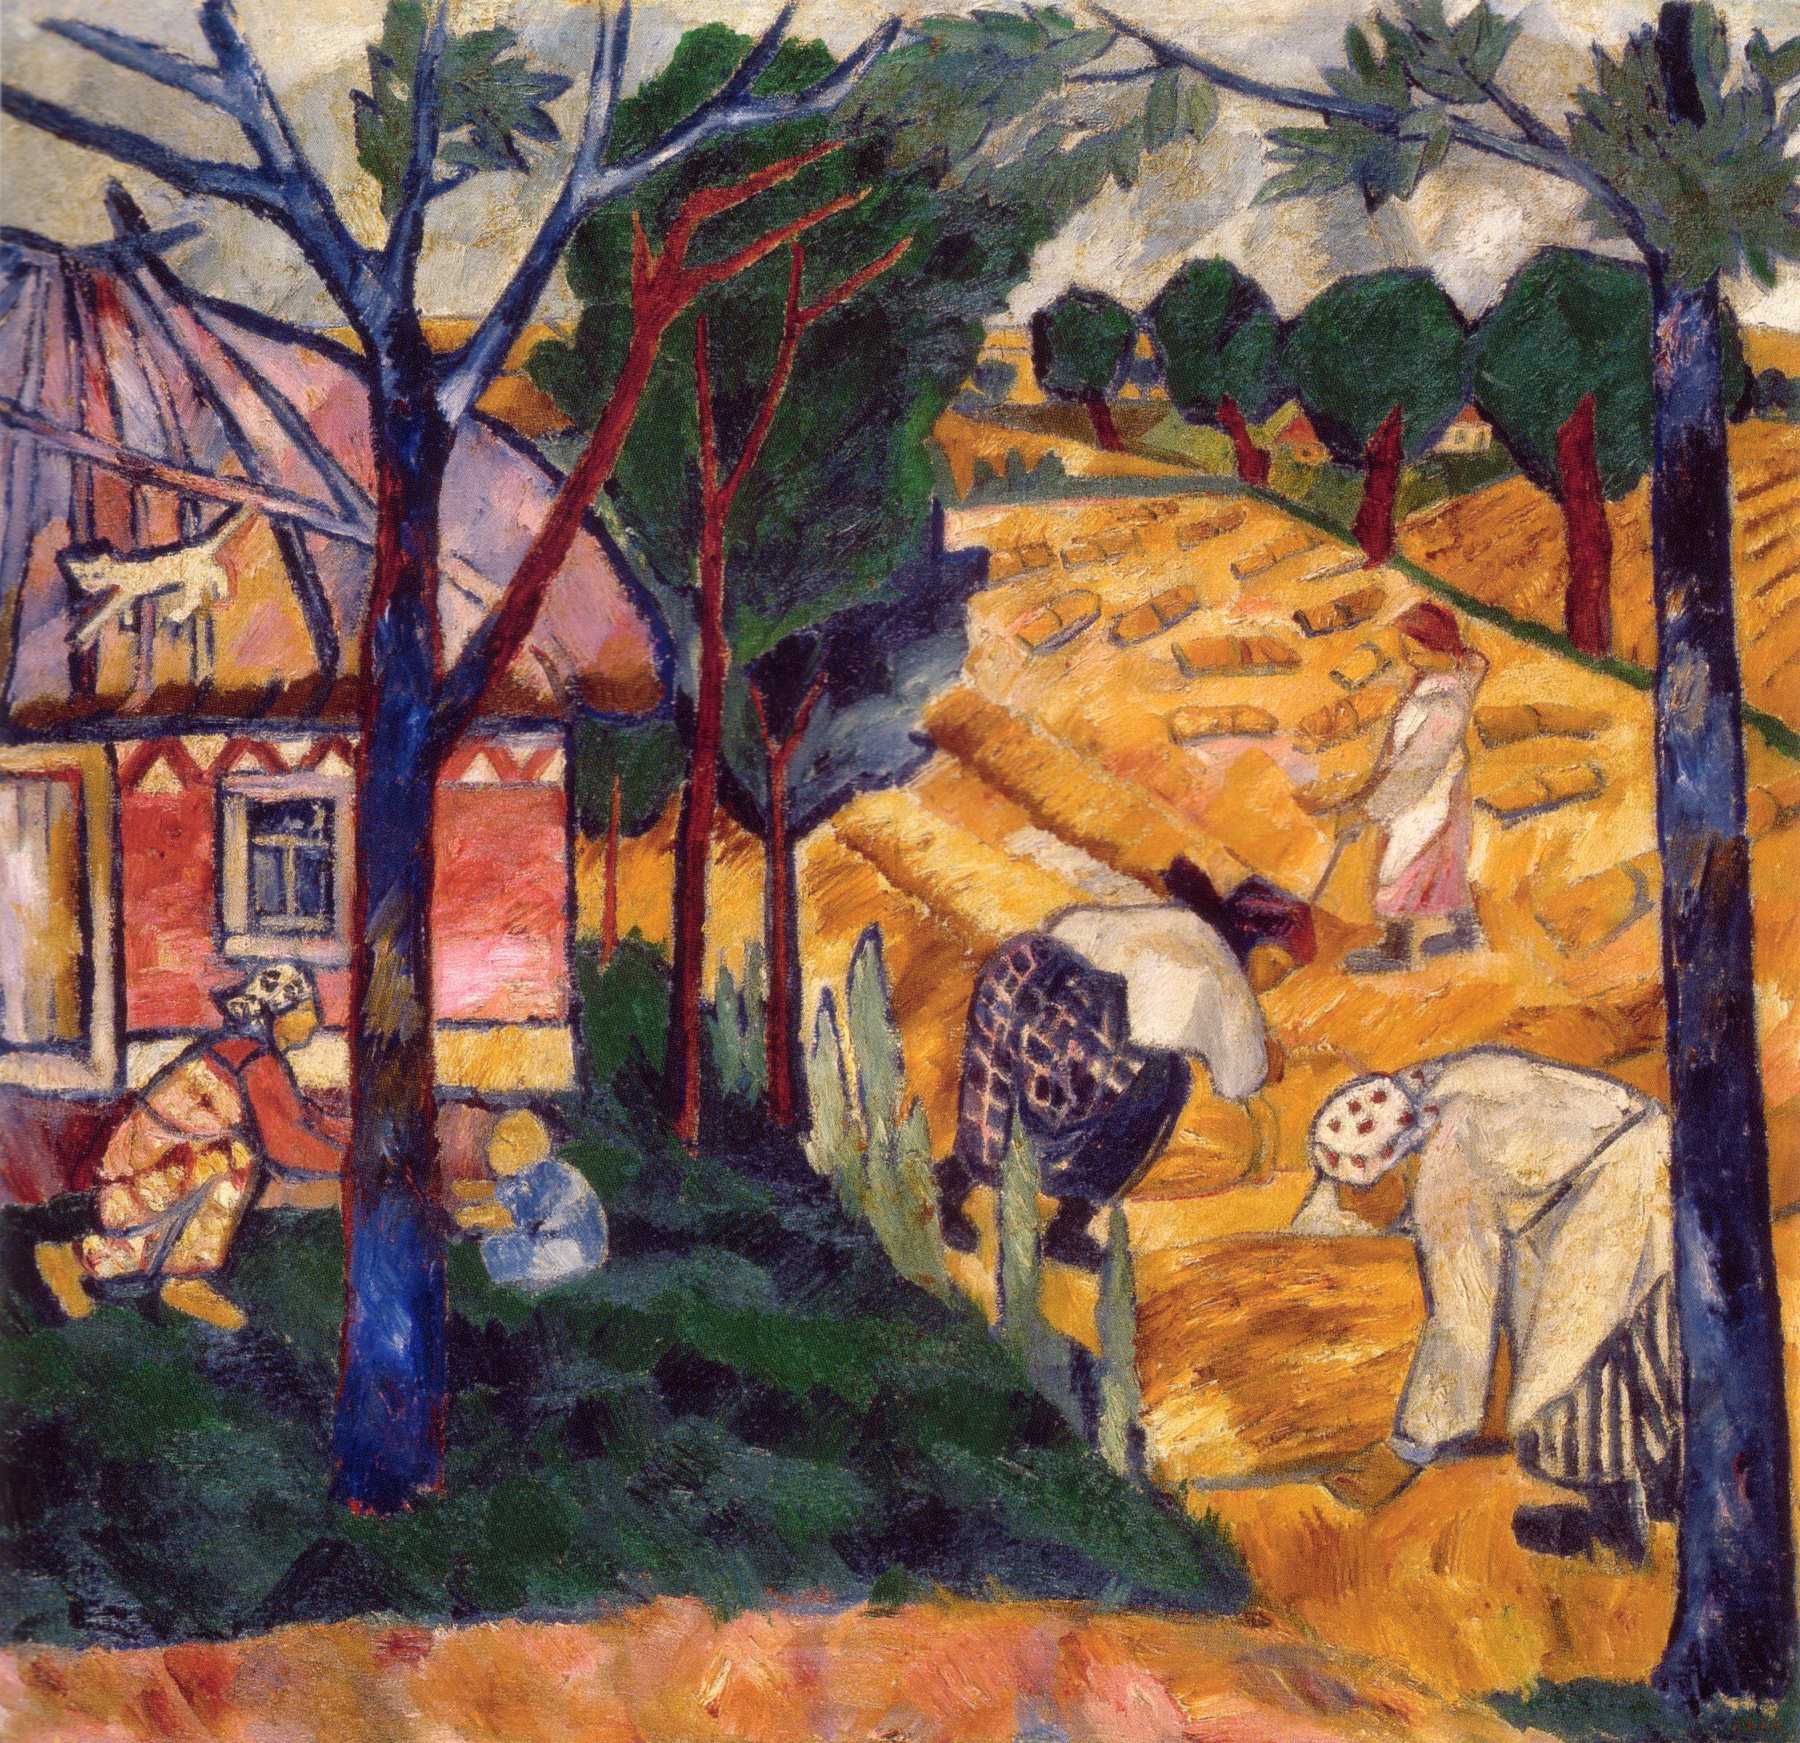
\includegraphics[height=1.1\paperheight]{./goncharova-harvesting.jpg}};
  \node[yshift=-5.5cm] at (current page.north) [text width=13cm, text height=8cm, fill=titlepagebackground] {};
  \node[yshift=-5.5cm] at (current page.north) [text width=12.7cm, text height=7.7cm, draw=wheat, line width=0.08cm] {};
  \node[yshift=-2.5cm, white] at (current page.north) {\huge\itshape\textsf{Lecture notes for the Master's course}};
  \node[yshift=-3.5cm, text=wheat] at (current page.north) {\HUGE\bfseries\OpenSansLight\textls{SHEAVES IN TOPOLOGY}};
  \node[yshift=-5cm, white] at (current page.north) {\LARGE\textsf{Taught at Utrecht University}};
  \node[yshift=-5.5cm, white] at (current page.north) {\LARGE\textsf{by Dr Remy van Dobben de Bruyn}};
  \node[yshift=-6.5cm, white] at (current page.north) {\LARGE\textsf{Notes by Ben Mason, Marcel Masqué Salgado,}};
  \node[yshift=-7cm, white] at (current page.north) {\LARGE\textsf{and Splinter Suidman}};
  \node[yshift=-8cm, white] at (current page.north) {\LARGE\textsf{Spring 2024}};
  \node[yshift=-8.5cm, white] at (current page.north) {\Large\textsf{Last update: \today}};
\end{tikzpicture}
\clearpage
\end{titlingpage}

\frontmatter
\pagestyle{plain}

\tableofcontents

\mainmatter
\aliaspagestyle{cleared}{plain}
\chapter*{Introduction}

These notes are based on lectures given by Remy van Dobben de Bruyn for the Master's course \emph{Sheaves in Topology}, taught at Utrecht University in the spring semester of 2023--2024.\footnote{See~\url{https://cursusplanner.uu.nl/course/WISM501/2023/SEM2} for the course description.}

The prerequisites for this course are a solid understanding of point-set topology, basic knowledge of fundamental groups and covering spaces, familiarity with the language of categories, and a working knowledge of modules over rings. 

\section*{Recommended literature}
Standard works:
\NewDocumentCommand\citeauthortitlecite{om}{\citeauthor{#2}, \citetitle{#2}~\IfNoValueTF{#1}{\cite{#2}}{\cite[#1]{#2}}}
\begin{itemize}
\item \citeauthortitlecite{IversenCohomologyOfSheaves}
\item \citeauthortitlecite{BredonSheafTheory}
\item \citeauthortitlecite{TennisonSheafTheory}
\item \citeauthortitlecite{KashiwaraSchapiraSheavesOnManifolds}
\item \citeauthortitlecite[\href{https://stacks.math.columbia.edu/tag/006A}{Chapter~006A}]{stacks-project} (chapter on sheaves)
\end{itemize}
\noindent
More advanced texts:
\begin{itemize}
\item \citeauthortitlecite{DimcaSheavesInTopology}
\item \citeauthortitlecite{MacLaneMoerdijkSheavesGeometryLogic}
\end{itemize}
\noindent
Exodromy correspondence (research papers):
\begin{itemize}
\item \citeauthortitlecite{TreumannExitPathsConstructibleStacks}
\item \citeauthortitlecite{CurryPatelClassificationConstructibleCosheaves}
\end{itemize}
\section*{Course content}
The first four lectures introduce presheaves and sheaves on a topological space $X$ and describe an equivalence of categories between local homeomorphisms over $X$ and sheaves on $X$. For the special case of locally constant sheaves there is an equivalence to the category of covering spaces of $X$. 

Some categorical properties of sheaves, and constructions such as the pushforward and the pullback, are discussed next. After an introduction to homological algebra (which is independent of the content on sheaves), the notion of sheaf cohomology is treated. This takes up \cref{lecture:8}, \cref{lecture:9}, \cref{lecture:10}, \cref{lecture:11}, and \cref{lecture:12}. 

The real fun begins when the homological algebra is applied to sheaves of abelian groups. One of the main results of the course, the proper base change theorem, is proven in \cref{lecture:15} for paracompact Hausdroff and locally compact Hausdorff spaces. The treatment of sheaf cohomology ends with a discussion of Čech cohomology. 

The last three weeks (\cref{lecture:18}, \cref{lecture:19}, \cref{lecture:20}) are reserved entirely to having fun, and as such were not examinable material in the 2024 version of the course. \todo{write after we write \cref{lecture:19}.} 

\todo{course content}


\chapter{Motivation, sheaves and presheaves}\label{lecture:1}

% \section{Introduction}
% \todo{Not sure if we want to add the examples etc.}


\section{Sheaves and presheaves}

\begin{defn}
    Let $X$ be a topological space. Write \indexterm{$\open(X)$} for the partially ordered set of opens of $X$.  A \indexdefnemph{presheaf} of sets on $X$ is a functor
    $
        F: \open(X)\opp \to \catSet. 
    $
\end{defn}
By changing the codomain we can obtain, for example, presheaves of abelian groups. In this course, we will focus almost entirely on presheaves of sets and of abelian groups.
Let $U \subset V $ be open sets of $X$. The inclusion under $F$ gives a \indexdefnemph{restriction} map $F(V) \to F(U)$. The naming comes from the following example: 

\begin{exmp}\label{exmp:ct-maps-presheaf}
    Let $X$ and $Z$ be topological spaces. The assignment $h_Z: \open(X)\opp \to \catSet$ by $U \mapsto \cont(U,Z)$ can be turned into a presheaf: given $U \subseteq V$ opens of $X$, define $$r_{UV}: \cont(V,Z) \to \cont(U,Z)$$ by $f \mapsto f|_U$.
\end{exmp}
We generalise the notation of function restriction. For $F(V) \to F(U)$, we denote the map pointwise by $s \mapsto s|_U$.

\begin{defn}\label{defn:sheaf}
    Let $X$ be a topological space and $\mathcal{F}: \open(X)\opp \to \catSet$ a presheaf on $X$.  We call $\mathcal{F}$ a \indexdefnemph{sheaf} if it satisfies the \emph{sheaf condition}\index{sheaf!sheaf condition}, i.e., if
    for every open $U \subset X$ and every open cover $(U_i)_{i \in I}$ of $U$ with $\bigcup_i U_i = U$, the map 
        \[
            \mathcal{F}(U) \to \prod_{i\in I}\mathcal{F}(U_i)\text{,} \quad s \mapsto (s|_{U_i})_{i \in I}
          \]
    \begin{enumerate}
        \item\label{defn:sheaf:injective} is injective, and
        \item\label{defn:sheaf:gluing} its image satisfies a \indexdefnemph{gluing condition}: it is given by $\setpred{(s_i)_{i\in I}}{s_i |_{U_i \cap U_j} = s_j | _ {U_i \cap U_j} \forall i,j \in I}$.
    \end{enumerate}
\end{defn}

\begin{rmk}\label{rmk:sheafs-as-equalizers}
    One checks that the sheaf condition is equivalent to requiring that
\[\begin{tikzcd}
	{\mathcal{F}(U)} & {\prod_i\mathcal{F}(U_i)} & {\prod_{i,j}\mathcal{F}(U_i \cap U_j)}
	\arrow[from=1-1, to=1-2]
	\arrow["\alpha", shift left, from=1-2, to=1-3]
	\arrow["\beta"', shift right, from=1-2, to=1-3]
\end{tikzcd}\]
    is an \indexterm{equaliser} diagram for all $U$ open in $X$ and for all $(U_i)_{i \in I}$ open covers of $U$ , where $\alpha: (s_i)_{i \in I} \mapsto s_i|_{U_i \cap U_j}$ and $\beta: (s_i)_{i \in I} \mapsto s_j|_{U_i \cap U_j}$.
\end{rmk}

\begin{lem} \label{lem:ct-maps-sheaf}
    The presheaf $h_Z$ from \cref{exmp:ct-maps-presheaf} is a sheaf.
\end{lem}
\begin{proof}
    If two functions agree on every open of a cover of $U$ they agree on $U$, this gives \cref{defn:sheaf}\cref{defn:sheaf:injective}. For~\cref{defn:sheaf:gluing}, we use the pasting lemma.
\end{proof}

\begin{exmp}
    Let $Z$ be a discrete topological space, let $X$ be a topological space. Given an open subset $U$ of $X$, a map $f: U \to Z$ is continuous if and only if it is locally constant. The sheaf $h_Z$ is called the \indexdefnemph{constant sheaf} on the set $Z$, labelled $\constSheaf{Z}$ or $\constSheaf{Z}_X$.
    Explicitly, \(\constSheaf{Z}\) is given by
    \[ \constSheaf{Z} \colon U \mapsto \cont(U,Z)\text{,} \]
    where \(Z\) is endowed with the discrete topology.
\end{exmp}

\begin{exmp}
    If $X$ is a \indexterm{manifold}, then the assignment $U \mapsto C^\infty(U, \mathbb{R})$ is a sheaf of $\mathbb{R}$ vector spaces. One can show that the assignment $U \mapsto \Omega^k(U)$ (smooth differential $k$-forms) is a sheaf.
\end{exmp}

\begin{lem}[name=sheaf of sections]\label{exmp:sheaf-of-sections}
    Let $f: Y \to X$ be a continuous map of topological spaces. The assignment on opens of $X$ given by 
    \[
        h_{Y/X}: U \mapsto \setpred{s: U \to f^{-1}(U) }{ f \circ s = \id_U} =: \cont[X](U, Y)
    \]
    is a sheaf.
\end{lem}
\begin{proof}
    One can prove the above lemma in a similar way we proved \cref{lem:ct-maps-sheaf}. 
    Alternatively, consider the diagram 
    \[\begin{tikzcd}
	{\cont[X](U,Y)} & {\cont(U,Y)} \\
	{\{U \to X\}} & {\cont(U,X)}
	\arrow["{f \circ -}", from=1-2, to=2-2]
	\arrow[from=1-1, to=2-1]
	\arrow[from=2-1, to=2-2]
	\arrow[from=1-1, to=1-2]
	\arrow["\lrcorner"{anchor=center, pos=0.125}, draw=none, from=1-1, to=2-2]
\end{tikzcd}\]
    and check that it is a pullback. We will come back to this in more detail in later lectures. 
\end{proof}

The sheaf \(h_{Y/X}\) of the lemma is called the \emph{sheaf of sections}\index{sheaf!of sections}.
The example in the lemma above is why the elements of $\mathcal{F}(U)$ for an arbitrary sheaf \(\mathcal F\) are more generally also called \emph{sections}\index{section}. 

\begin{exmp}
    Let $f: Y \to X$ be the two-to-one cover of the circle\index{circle covering}: $f: z \mapsto z^2$, with $X := S^1$ and $Y:= S^1$. 
    On small intervals $U \subset X$ we get $f^{-1}(U)  \cong U \times \{1,2\}$. We thus have two sections: $U \mapsto (U, 1)$ and $U \mapsto (U, 2)$, so $h_{Y/X}(U)$ has two elements.
    On $V$ a union of small intervals, we get $2^{|\pi_0(V)|}$ elements, where $|\pi_0(V)|$ is the number of path components of $V$. 
    On $W = X$, we get no sections. If $s: X \to Y$ is a section, then the induced map $s_*: \pi_1(X) \to \pi_1(Y)$ is a section to the map $f_*: \pi_1(Y) \to \pi_1(X)$. But this induced map is multiplication by $2$, and it does not have a section. 
\end{exmp}

\chapter{Morphisms of (pre)sheaves, Yoneda lemma, étalé space}\label{lecture:2}

\remyquote{You can do what you want, it's a free world (on one generator).}
%% NOTE: You can do what you want [with respect to underlining/boldfacing names of categories]

\section{Morphisms of (pre)sheaves}

\begin{defn}
Let $\cat C$ be a small category.
Then \indexdefn{$\catPresheaf(\cat C)$} is the functor category $\catFunctor(\cat C\opp,\catSet)$: its objects are functors $F\colon\cat C\opp\to\catSet$, and its morphisms $\alpha\colon F\To G$ are \emph{natural transformations}\index{natural transformation}, that is, collections of functions $\alpha_X\colon F(X)\to G(X)$ for all $X\in\cat C$ such that the diagram
\begin{equation*}
    \begin{tikzcd}
        F(Y) \ar[r, "\alpha_Y"] \ar[d, "F(f)"'] & G(Y) \ar[d, "G(f)"] \\
        F(X) \ar[r, "\alpha_X"'] & G(X)
    \end{tikzcd}
\end{equation*}
commutes for all $f\colon X\to Y$ in $\cat C$.
\end{defn}

\begin{defn}
Let $X$ be a topological space.
Then the category of presheaves on $X$ is $\catPresheaf(X)\coloneqq\catPresheaf(\open(X))$\index{$\catPresheaf(X)$} and the category of sheaves on $X$ is the full subcategory $\catSheaf(X)\subseteq\catPresheaf(X)$\index{$\catSheaf(X)$} on the sheaves.
\end{defn}

\begin{lem}\label{lem:psh-category-set}
Let $\cat C$ be a small category.
Then:
\begin{enumerate}
\item $\catPresheaf(\cat C)$ is a category.
\item The category $\catPresheaf(\cat C)$ has all (small) limits\index{limit} and colimits\index{colimit}, and they are computed objectwise; e.g., for presheaves $F,G\in\catPresheaf(\cat C)$ the natural map
    \[ (F\times G)(U) \to F(U)\times G(U) \]
    is an isomorphism for all open $U\subseteq X$.
\item A natural transformation $\alpha\colon F\To G$ between presheaves $F$ and $G$ on $\cat C$ is invertible if and only if the component $\alpha_X\colon F(X)\to G(X)$ is a bijection for all $X\in\cat C$.
\end{enumerate}
\end{lem}

\begin{rmk}
Colimits\index{colimit} in the category $\catSheaf(X)$ of sheaves will be more complicated.
\end{rmk}

\begin{exmp}
Recall that we defined a sheaf $h_Z$ on $X$ for $Z\in\catTopologicalSpace$ (\cref{exmp:ct-maps-presheaf}).
If $g\colon Z\to Z'$ is a continuous map, then we get a natural transformation $h_Z\To h_{Z'}$ with component
\[ \cont(U,Z) \to \cont(U,Z')\text{,} \quad f \mapsto g\circ f \]
at $U\in\open(X)$.
One checks that this is natural.
\end{exmp}

\begin{exmp}
For the sheaf of sections (\cref{exmp:sheaf-of-sections}), a map $g\colon Y\to Y'$ over $X$ induces a natural transformation $h_{Y/X}\To h_{Y'/X}$ with component
\[ \cont[X](U,Y) \to \cont[X](U,Y')\text{,} \quad s \mapsto g\circ s \]
at $U\in\open(X)$.
This is again natural in $U$.
\end{exmp}

In fact, the sheaf $h_Z$ is a special case of $h_{Y/X}$:
\begin{lem}
If $Y=Z\times X\xrightarrow{\pr_X} X$ in $\catTopologicalSpace_{/X}$, then the sheaves $h_{Y/X}$ and $h_Z$ are isomorphic.
\end{lem}
\todo{Picture}
\begin{proof}
For $U\in\open(X)$, define
\[ \cont[X](U,Z\times X) \to \cont(U,Z)\text{,} \quad s\mapsto \pr*_Z\circ s \]
and
\[ \cont(U,Z) \to \cont[X](U,Z\times X)\text{,} \quad f \mapsto (u\mapsto (f(u),u))\text{.} \]
These maps are inverses.
Both transformations are natural. For the first: given an inclusion of opens $U\subseteq V\subseteq X$, the diagram
\begin{equation*}
    \begin{tikzcd}
        \cont[X](V,Z\times X) \ar[r, "\pr*_Z\circ -"] \ar[d, "(-)|_U"'] & \cont(V,Z) \ar[d, "(-)|_U"] \\
        \cont[X](U,Z\times X) \ar[r, "\pr*_Z\circ -"'] & \cont(U,Z)
    \end{tikzcd}
\end{equation*}
commutes.
\end{proof}

\begin{exmp}
Let $Y\to X$ be the two-to-one cover $\sphere[1]\to\sphere[1]$\index{circle covering}.
Then $h_{Y/X}$ is not isomorphic to $h_Z$ for any $Z\in\catTopologicalSpace$ (but it is locally isomorphic to $h_{\{1,2\}}$, as we will see later\todo{Ref back}).

Suppose $h_{Y/X}\cong h_Z$ for $Z\in\catTopologicalSpace$.
Then $Z\neq\emptyset$, for
\[ h_\emptyset(U) = \begin{cases}
    \emptyset & \text{if } U \neq\emptyset\text{,} \\
    \terminal & \text{if } U =\emptyset\text{.}
\end{cases} \]
But we have seen that $h_{Y/X}$ is nonempty for a small enough interval.
So $Z\neq\emptyset$, so constant maps show that $h_Z(U)\neq\emptyset$ for all $U$.
But last lecture, we saw that $h_{Y/X}(X)=\emptyset$.
\todo{Ref}
\end{exmp}

\section{Yoneda lemma}

\begin{defn}
Let $\cat C$ be a small category.
Then the \emph{representable presheaf}\index{presheaf!representable} on $X\in\cat C$ is the presheaf
\[ h_X \colon \cat C\opp\to\catSet\text{,} \quad Y \mapsto \Hom[\cat C](Y,X) \]
with restriction map
\[ f^*\colon\Hom[\cat C](X,Y')\to\Hom[\cat C](X,Y)\text{,} \quad g\mapsto g\circ f\text{.} \]
induced by $f\colon Y\to Y'$ in $\cat C$.
\end{defn}

\begin{rmk}
The sheaf $h_Z$ on $X$ from \cref{exmp:ct-maps-presheaf} is \emph{not} a representable presheaf on $\open(X)$.
The sheaf $h_Z$ sends an open $U\subseteq X$ to the set $\cont(U,Z)$ of all continuous  maps $U\to Z$, whereas the representable presheaf $h_V$ represented by an open $V\subseteq X$ sends $U\subseteq X$ to the set $\Hom[\open(X)](U,V)$ of inclusions $U\hookrightarrow V$ (a subsingleton set).
The sheaf $h_Z$ can be regarded as the \emph{restriction} of the representable presheaf $h_Z = \Hom[\catTopologicalSpace](-,Z)$ on the (non-small) category of spaces to the (non-full) subcategory $\open(X)\subseteq\catTopologicalSpace$.
\end{rmk}

In some sense, the representable presheaf represented by $X$ is `freely generated' by the section $\id_X\in h_X(X)$.

\begin{lem}[name={\indexdefn{Yoneda lemma}~\cite[Theorem~2.2.4]{riehlCategoryTheoryContext2016}}]\label{lem:yoneda}
    Let $F: \cat C\opp \to \catSet$ be a functor, $X \in \cat C$. Then the map \[
    \Phi: \Hom_{\catPresheaf(\cat C)}(h_X, F) \to F(X)\text{,} \quad \alpha\mapsto \alpha_X(\id_X)
    \] is a bijection that is natural in $F$ and $X$. 
\end{lem}
\begin{proof}
    We leave the naturality in $F$ and $X$ as an exercise. Part of the exercise is to work out what is meant by naturality in $F$ and $X$. \todo{maybe add details}
    The inverse of $\Phi$ will be a map \[
    \Psi: F(X) \to \Hom_{\catPresheaf(C)}(h_X, F)
    \] defined by $s \mapsto (f \mapsto F(f)(s))_{Y \in \cat C}$.
    The first thing to check is that this map lands in $\Hom_{\catPresheaf(\cat C)}(h_X, F)$. That is, we need to check $\Psi(s)$ is a natural transformation. This is true: given $g: Y \to Z$ in $\cat C$ the diagram 
    \[
    \begin{tikzcd}
{\Hom(Z,X)} \arrow[d, "-\circ g"'] \arrow[r, "\Psi(s)_Z"] & F(Z) \arrow[d, "F(g)"] \\
{\Hom(Y,X)} \arrow[r, "\Psi(s)_Y"']                       & F(Y)            
\end{tikzcd}
    \] commutes, since we have $F(g)(\Psi(s)_Z(f)) = F(g)(F(f)(s)) = F(fg)(s) = \Psi(s)_Y(fg)$.
    We check that $\Psi$ provides an inverse for $\Phi$. One side is immediate: $\Phi \Psi(s) = \Psi(s)_X(\id_X) = F(\id_X)(s) = s$. 
    For the converse, let $\alpha: h_X \to F$ be a natural transformation. We check that $\Psi \Phi(\alpha) = \alpha$. 
    Let $Y \in \cat C$, and $f \in \Hom(Y, X)$. The naturality of $\alpha$ gives a commutative diagram
    \[
    \begin{tikzcd}
{\Hom(X,X)} \arrow[d, "-\circ f"'] \arrow[r, "\alpha_X"] & F(X) \arrow[d, "F(f)"] \\
{\Hom(Y,X)} \arrow[r, "\alpha_Y"']                        & F(Y)                  
\end{tikzcd}
\] We now have $\Psi(\Phi \alpha)_Y(f) = F(f)(\Phi \alpha) = F(f) (\alpha_X(\id_X)) = \alpha_Y (\id_X \circ f)= \alpha_Y(f)$ by plugging in $\id_X$ into the diagram above. 
\end{proof}

\section{Étalé space}

In the coming lectures, we will show that every sheaf on a space $X$ is isomorphic to $h_{Y/X}$ for some map $Y\to X$.
We will construct a functor $\etalespace*\colon\catPresheaf(X)\to\catTopologicalSpace_{/X}$ which sends a presheaf to its \emph{étalé space} (also called \emph{espace étalé}\index{espace étalé|see{étalé space}}, (wrongly) \emph{étale space} or \emph{sheaf space} (but we do not like that)).

The idea is as follows: a presheaf $F$ is determined by its values $F(U)$ for opens $U\subseteq X$ and the restriction maps.
By the Yoneda lemma, the values can be written as $F(U)\cong\Hom[\catPresheaf(X)](h_U,F)$.
For $h_U$, the étalé space will be the space $U\to X$ over $X$.
In general, a presheaf $F$ is `generated by copies of $h_U$ modulo relations from the restrictions'.
We define $\etalespace(F)\to X$ by glueing copies of $U$ `along the same colimit diagram' (but now in $\catTopologicalSpace_{/X}$ instead of $\catPresheaf(X)$).

\begin{defn}\label{defn:espace-étalé}
Let $F$ be a presheaf on $X$.
The \indexdefnemph{étalé space} $\etalespace(F)$ is the quotient of the coproduct
\[ \coprod_{U\in\open(X)} F(U)\times U \]
(where $F(U)$ is endowed with the discrete topology), with notation $(s,x)_U$ for the point given by $s\in F(U)$ and $x\in U$ in the factor indexed by $U$, by the equivalence relation generated by
\[ (s|_U, x)_U \sim (s, x)_V \]
for $(s,x)\in F(V)\times U$ for $x\in U\subseteq V$.
\end{defn}

Categorically, the étalé space is the \indexterm{coequaliser}
\[ \etalespace(F) = \coeq\bigl(\coprod_{U\subseteq V\subseteq X} F(V)\times U \rightrightarrows \coprod_{U\subseteq X} F(U)\times U\bigr)\]
where the arrows are given by
\begin{equation*}
    \begin{tikzcd}[row sep=tiny]
        F(U)\times U & F(V)\times U \ar[l, "\incl*^*\times\id"'] \ar[r, "\id\times \incl*"] & F(V)\times V \\
        (s|_U, x) \ar[u, "\in", phantom, marking] & (s,x) \ar[l, mapsto] \ar[r, mapsto] \ar[u, "\in", phantom, marking] & (s,x) \ar[u, "\in", phantom, marking]
    \end{tikzcd}
\end{equation*}
where $\incl*\colon U\hookrightarrow V$ denotes the inclusion map.

Alternatively, the étalé space $\etalespace(F)$ is the \indexterm{coend}
\[ \etalespace(F) = \int^{U\in\open(X)} F(U)\times U\text{.} \]

To understand the étalé space a bit better, we have to understand the equivalence relation generated by the given relation, with respect to which we take the quotient.

\begin{rmk}\label{rmk:equivalence-relation-generated}
Let $\sim$ be a relation on a set $X$.
The equivalence relation $\approx$ on $X$ generated by $\sim$ can be explicitly defined as follows: we say $x\approx y$ if and only if there is a finite zigzag
\begin{equation*}
    \begin{tikzcd}
        & a_1 & & a_3 & & a_{2n-1} \\
        x = a_0 \ar[ru, "\sim"] & & a_2 \ar[lu, "\sim"'] \ar[ru, "\sim"] & & \ldots \ar[lu, "\sim"'] \ar[ru, "\sim"] & & a_{2n}=y \ar[lu, "\sim"']
    \end{tikzcd}
\end{equation*}
of elements $a_i\in X$ such that $x=a_0$, $y=a_{2n}$, $a_{2i}\sim a_{2i+1}$ for $0\leq i<n$ and $a_{2i}\sim a_{2i-1}$ for $0<i\leq n$.
\end{rmk}

\begin{exmp}
To compute the \indexterm{coequaliser} of the diagram of sets
\begin{equation*}
    \begin{tikzcd}
        \{1,2\} \ar[r, shift left, "-\cdot 1"] \ar[r, shift right, "-\cdot 2"'] & \{1,2,3,4\}
    \end{tikzcd}
\end{equation*}
where the maps multiply by one and two, respectively, we need to understand the equivalence relation generated by $x\sim 2x$ for all $x\in\{1,2\}$.
That is, we have $1\sim 2$ and $2\sim 4$, and nothing more.
The equivalence classes in the relation $\approx$ generated by $\sim$ then are $\{1,2,4\}$ and $\{3\}$.
\end{exmp}

\begin{lem}
If $(s,x)_U\in F(U)\times U$ and $(t,y)_V\in F(V)\times V$, then $(s,x)_U\approx (t,y)_V$ (that is, they are equivalent under the equivalence relation generated by $\sim$ as in \cref{defn:espace-étalé}) if and only if $x = y$ and there exists an open neighbourhood $W\subseteq U\cap V$ of $x$ such that $s|_W = t|_W$.
\end{lem}

One can prove this lemma using the explicit description of $\approx$ given in \cref{rmk:equivalence-relation-generated}, but this is difficult combinatorics!
A better proof shows that the relation on the right in the equivalence of the lemma is an equivalence relation and that the former statement implies the latter (i.e., `$\sim$ implies $\approx$').

\begin{exmp}\label{exmp:representable-presheaf-espace-étalé}
If $F = h_U$ is the representable presheaf\index{presheaf!representable} on $X$ represented by an open $U\subseteq X$ (see \cref{fig:presheaf-represented-by-U}), then
\[ F(V) = \Hom[\open(X)](V,U) = \begin{cases}
    \terminal & \text{if } V\subseteq U\text{,} \\
    \emptyset & \text{if } V\not\subseteq U\text{.}
\end{cases}\]
The étalé space $\etalespace(F)$ is the quotient of
\[ \coprod_{V\subseteq X} F(V)\times V = \coprod_{V\subseteq U} V \]
by the equivalence relation generated by $(*,x)_V\sim(*,x)_{V'}$ for all $V,V'\subseteq U$.
This just leaves $U$, so $\etalespace(h_U) = U$.
\end{exmp}

\begin{figure}
    \centering
    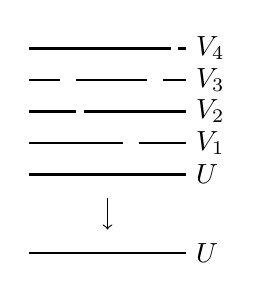
\begin{tikzpicture}
        \node (U) at (2, 0) [right] {\(U\)};
        \node (U') at (2, 1) [right] {\(U\)};
        \node (V1) at (2, 1.4) [right] {\(V_1\)};
        \node (V2) at (2, 1.8) [right] {\(V_2\)};
        \node (V3) at (2, 2.2) [right] {\(V_3\)};
        \node (V4) at (2, 2.6) [right] {\(V_4\)};
        \draw[thick] (0, 0) -- (2, 0);
        \draw[thick] (0, 1) -- (2, 1);
        \draw[thick] (0, 1.4) -- (1.2, 1.4); \draw[thick] (1.4, 1.4) -- (2, 1.4);
        \draw[thick] (0, 1.8) -- (0.6, 1.8); \draw[thick] (0.7, 1.8) -- (2, 1.8);
        \draw[thick] (0, 2.2) -- (0.4, 2.2); \draw[thick] (0.6, 2.2) -- (1.5, 2.2); \draw[thick] (1.7, 2.2) -- (2, 2.2);
        \draw[thick] (0, 2.6) -- (1.8, 2.6); \draw[thick] (1.9, 2.6) -- (2, 2.6);
        \draw[->] (1, .7) -- (1, .3);
    \end{tikzpicture}
    \caption{The presheaf $F = h_U$ represented by $U\subseteq X$ of \cref{exmp:representable-presheaf-espace-étalé}.}
    \label{fig:presheaf-represented-by-U}
\end{figure}

\begin{rmk}
In general, the étalé space $\etalespace(F)$ is not `computable'.
It is, however, when $F$ is \emph{constructible}\index{constructible sheaf}, which we will see in one of the final lectures.\todo{Ref back}
\end{rmk}

\begin{prop}
    The construction of the étalé space defines a functor
    $\catSheaf(X) \to \catTopologicalSpace_{/X}$.
\end{prop}
\begin{proof}
    We can cheat and use the unproven remark that the étalé space is a \indexterm{coend}. \todo{prove?}
\end{proof}

\subfile{Lectures/Lecture 3}
\chapter{Sheafification, monodromy}\label{lecture:4}

\section{Sheaf/space adjunction (continued)}
\remyquote{Computers don't have noses.}
\noindent
We still have to prove that the counit of the sheaf/space adjunction is an isomorphism for local homeomorphisms to prove the equivalence $\catSheaf(X)\simeq\catLocalHomeomorphism_{/X}$.

\begin{proof}[of the restricted equivalence in \cref{thm:sheaf-space-adjunction}, continued]
If $f\colon Y\to X$ is a local homeomorphism, we have to show that the counit
\[ \epsilon_{Y/X} \colon \etalespace(h_{Y/X}) \to Y \]
is an isomorphism in $\catLocalHomeomorphism_{/X}$ (or $\catTopologicalSpace_{/X}$).
Concretely, this map is given by
\begin{equation*}
    \begin{tikzcd}[column sep=small]
        \coprod_{U\subseteq X}\cont[X](U,Y)\times U \ar[rr] \ar[rd, epi] & & Y \\
        & \etalespace(h_{Y/X}) \ar[ru, "\epsilon_{Y/X}"']
    \end{tikzcd}
\end{equation*}
where the top map sends $(s,x)_U$ to $s(x)\in Y$.
This map indeed descends to the étalé space $\etalespace(h_{Y/X})$: if $x\in U\subseteq V$ and $s\colon V\to Y$ is a section, then $(s,x)_V\sim(s|_U,x)_U$, and both are sent to $s(x)$.

By \cref{lem:localhomtriangle,lem:etalelocalhomeo}, the map $\etalespace(h_{Y/X})\to Y$ is a local homeomorphism, so in particular an open map, so it suffices to check that it is bijective.

For injectivity, assume $\epsilon_{Y/X}([s,x]_U)=\epsilon_Y([t,y]_V)$.
Then $x=y$ since everything is over $X$, and thus \(s(x)=t(x)\) by assumption.
Let \(S\) be an open neighbourhood of \(s(x)=t(x)\) in \(Y\) such that \(f\) restricts to a homeomorphism \(f|_S\colon S\to f(S)\), and set \(W\coloneq s\inv(S)\cap t\inv(S)\).
Observe that \(W\) contains \(x\).
Then \(s|_W\) and \(t|_W\) are both sections to the injective map \(f|_S\colon S\hookrightarrow X\), so they agree.
Hence \((s,x)_U\approx(s|_W,x)_W=(t|_W,x)_W\approx(t,x)_V\) and we conclude that \(\epsilon_{Y/X}\) is injective.

For surjectivity, let \(y\in V\) and set \(x=f(y)\in X\).
Choose an open neighbourhood \(V\subseteq Y\) of \(y\) such that \(f\) restricts to a homeomorphism \(f|_V\colon V\to f(V) \eqcolon U\) onto an open subset.
Write \(s\colon U\to V\) for its inverse \(f|_V\inv\); then \(s\colon U\to V\subseteq Y\) is a section with \(s(x)=y\), so \(\epsilon_{Y/X}([s,x]_U)=y\), showing that \(\epsilon_{Y/X}\) is surjective.

We conclude that the counit of the sheaf/space adjunction is an isomorphism for local homeomorphisms, finishing the proof of the equivalence of categories \(\catSheaf(X)\simeq\catLocalHomeomorphism_{/X}\) of \cref{thm:sheaf-space-adjunction}.
\end{proof}

\begin{defn}
For a space $X$, the composite functor
\[ (-)^\sharp \coloneq h_{-/X} \circ \etalespace* \colon \catPresheaf(X)\to\catSheaf(X) \]
is called \indexdefnemph{sheafification}.
It comes with a natural map $F\To F^\sharp$ for presheaves $F$ on $X$ given by the unit of the adjunction $\etalespace*\leftadj h_{-/X}$.
\end{defn}

The following result can be seen as the universal property of sheafification\index{sheafification!universal property}.

\begin{cor}\label{cor:sheafification-left-adjoint-to-inclusion}
Sheafification is left adjoint to the inclusion $\catSheaf(X)\hookrightarrow\catPresheaf(X)$.
That is, if $F$ is a presheaf on $X$ and $\mathcal G$ is a sheaf on $X$, then every map $F\To \mathcal G$ of presheaves factors uniquely through the natural map $F\To F^\sharp$.
\end{cor}
\begin{proof}
Compose the adjunction $\etalespace*\leftadj h_{-/X}$ and the equivalence $\catLocalHomeomorphism_{/X}\simeq\catSheaf(X)$.
\end{proof}

The unit of the adjunction is the map $F\To F^\sharp$; it is an isomorphism if and only if $F$ is a sheaf.

\begin{exmp}\label{exmp:sheaf-on-point-set}
For the one-point space $*$, we have $\open(*) = \{\emptyset\hookrightarrow *\}$, so
\[ \catPresheaf(X) = \catFunctor(\mathord{\to},\catSet) \]
is the arrow category of $\catSet$.
As we have seen in the homework, a presheaf $F$ on the one-point space -- that is, a map $F(*)\to F(\emptyset)$ -- is a sheaf if and only if $F(\emptyset)=*$.
Hence we have an equivalence $\catSheaf(X)\simeq\catSet$.
Of course, we also have $\catLocalHomeomorphism_{/*} \simeq\catSet$ since having a local homeomorphism $X\to *$ implies $X$ is discrete.
\end{exmp}

\begin{exmp}
Let $S=\{0,1\}$ be the \indexterm{Sierpiński space} with
\[ \open(S) = \{\emptyset\hookrightarrow\{1\}\hookrightarrow S\}\text{.} \]
Using a similar argument as in the previous example, we see
\[ \catPresheaf(S) \simeq \catFunctor(\mathord{\to}\mathord{\to},\catSet) \]
and
\[ \catSheaf(S) \simeq \catFunctor(\mathord{\to},\catSet)\text{.} \]
\end{exmp}

\begin{exc}
Check that sheafification on $S$ is given by sending a presheaf $F$ -- that is, a pair of maps $F(S)\to F(\{1\})\to F(\emptyset)$ -- to the sheaf given by the map $F(S)\to F(\{1\})$.
\end{exc}

\section{Restriction of sheaves}
\remyquote{You can do this for different values of four, here we do it for five.}

\begin{defn}
Let $U\subseteq X$ be open and let $F$ be a presheaf on $X$.
Then the \emph{restriction}\index{restriction!of sheaves} $F|_U$ of $F$ to $U$ is the restriction of the functor $F$ along the inclusion $\open(U)\hookrightarrow\open(X)$.
\end{defn}

\begin{lem}
If $\mathcal F$ is a sheaf on $X$, then so is its restriction $\mathcal F|_U$ to an open $U\subseteq X$.
Under the equivalence $\catSheaf(X)\simeq\catLocalHomeomorphism_{/X}$, restriction to $U$ corresponds to sending a local homeomorphism $f\colon Y\to X$ to the \indexterm{pullback} $f\inv(U)\to U$.
\end{lem}

In $\catLocalHomeomorphism_{/X}$, we have the subcategory $\catCoveringSpace_{/X}$ of \emph{covering spaces}\index{covering space}: continuous maps $f\colon Y\to X$ such that $X$ has an open cover $X = \bigcup_{i\in I}U_i$ and there are sets $S_i$ such that $f\inv(U_i)\to U_i$ is isomorphic to $U_i\times S_I\to U_i$ (where $S_i$ has the discrete topology) over $U_i$ for all $i\in I$.

\todo{Pancake example}

\begin{rmk}
We will not assume that the space $Y$ in a covering space $Y\to X$ is (path) connected; this condition does appear in the literature with some authors.
\end{rmk}

\begin{defn}
A sheaf $\mathcal F$ on a space $X$ is \emph{locally constant}\index{sheaf!locally constant} if there is an open cover $X = \bigcup_{i\in I}U_i$ such that the restriction $\mathcal F|_{U_i}$ is a constant sheaf $h_{S_i}$ for some set $S_i$ for all $i\in I$.

We write $\catLocallyConstantSheaf(X)$ for the full subcategory of $\catSheaf(X)$ on the locally constant sheaves.
\end{defn}

\begin{lem}
Under the equivalence $\catSheaf(X)\simeq\catLocalHomeomorphism_{/X}$, the locally constant sheaves correspond to covering spaces.
In other words, this equivalence restricts to an equivalence
\[ \catLocallyConstantSheaf(X) \simeq \catCoveringSpace_{/X}\text{.} \]
\end{lem}

The real content is the constant case: we have $\mathcal F\cong h_S = h_{X\times X/X}$ if and only if $\etalespace(\mathcal F)\cong X\times S$ over $X$.
% \begin{proof}
% First, let $\mathcal F$ be a locally constant sheaf on $X$.
% Then there is an open cover $X = \bigcup_{i\in I}U_i$ such that $\mathcal F|_{U_i}\cong h_{S_i}$ for some set $S_i$ for all $i\in I$.
% \end{proof}

\todo{Four-to-one cover of the circle example}

\section{Review of monodromy}
\remyquote{If you've ever been in a parking garage, you know what I mean.}

\begin{figure}[h!]
  \centering
  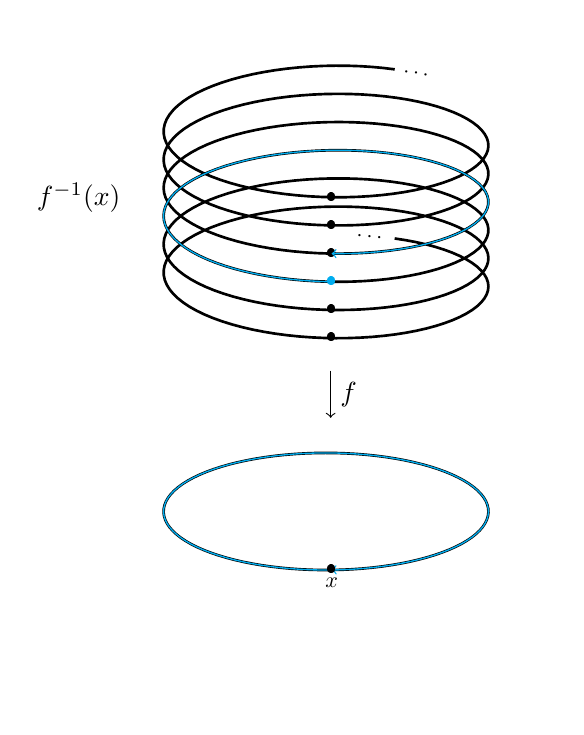
\begin{tikzpicture}[scale=.8]
    \begin{axis}[axis line style={draw=none}, tick style={draw=none}, xticklabel=\empty, yticklabel=\empty, zticklabel=\empty]
      \addplot3+[domain=0:12*pi,samples=500,samples y=0,black,no marks,very thick]
        ({sin(deg(x))}, {cos(deg(x))}, {6*x/(pi)})
        node[pos=0, left, rotate=-5] {\ldots}
        node[pos=1, right, rotate=-10] {\ldots}
        node[pos=0.85/12] {\textbullet}
        node[pos=2.85/12] {\textbullet}
        node[pos=6.85/12] {\textbullet}
        node[pos=8.85/12] {\textbullet}
        node[pos=10.85/12] {\textbullet};
      \addplot3+[domain=4.85*pi:6.85*pi,samples=500,samples y=0,cyan,no marks,semithick,->] ({sin(deg(x))}, {cos(deg(x))}, {6*x/(pi)}) node[pos=0] {\textbullet};
    \end{axis}
    \node at (-0.5,3) {\(f^{-1}(x)\)};
    \draw[->] (3.5,.25) -- (3.5,-0.5) node[right] at (3.5,-0.125) {\(f\)};
    \begin{axis}[axis line style={draw=none}, tick style={draw=none}, xticklabel=\empty, yticklabel=\empty, zticklabel=\empty, at={(0,0,-300)}]
      \addplot3+[domain=0.85*pi:2.85*pi,samples=100,samples y=0,black,no marks,very thick]
        ({sin(deg(x))}, {cos(deg(x))}, {0});
      \addplot3+[domain=0.85*pi:2.85*pi,samples=100,samples y=0,cyan,no marks,semithick,->]
        ({sin(deg(x))}, {cos(deg(x))}, {0})
        node[pos=0,black] {\textbullet}
        node[pos=0,black,below] {\(x\)};
    \end{axis}
  \end{tikzpicture}
  \caption{Unique path lifting in the cover of the circle by the helix}
  \label{fig:unique-path-lifting-circle-helix}
\end{figure}

\begin{defn}
    Let $X$ be a topological space. Then $X$ is 
    \begin{enumerate}
        \item \emph{locally path connected} if every open neighbourhood $x \in U$ of any $x \in X$ contains a path connected open neighbourhood $x \in V \in U$.
        \item \emph{semi-locally path connected} if for every $x \in X$, there exists an open neighbourhood $x\in U$ such that the map $\homotopy[1](U, x) \to \homotopy[1](X,x)$ is trivial. 
    \end{enumerate}
\end{defn}

\begin{defn}
    Let $X$ be a topological space and $x\in X$. The \indexdefnemph{fibre functor} is defined by
    \begin{align*}
        F_x: \catCoveringSpace_{/X} &\to \homotopy[1](X,x)\catSet\\
        (Y \xrightarrow{f} X) &\mapsto f^{-1}(x),
    \end{align*}
    where a loop $\gamma \in \homotopy[1](X,x)$ acts on $f^{-1}(x)$ by unique path lifting. 
\end{defn}

\begin{thm}[name={\indexterm{monodromy} correspondence}]
    Let $X$ be a topological space and $x \in X$. 
    \begin{enumerate}
        \item If $X$ is path connected and locally path connected, then
        \[
            F_x: \catCoveringSpace_{/X} \to \homotopy[1](X,x)\catSet
        \] is fully faithful. 
        \item If $X$ is moreover semi-locally simply connected, then $F_x$ is an equivalence of categories. 
    \end{enumerate}
\end{thm}
\begin{proof}[outline]\todo{Maybe type up the details Marcel}
    \begin{itemize}
        \item Any covering $f: Y \to X$ is locally path connected (easy). It is furthermore a disjoint union $\coprod_{i \in I} Y_i$ of path connected spaces $Y_i$ \cite[Theorem~25.4]{MunkresTopology}.
        \item Any map $Y \xrightarrow{\phi}Y' \in \catCoveringSpace_{/X}$ is itself a covering \cite[Lemma~80.2(a)]{MunkresTopology}.
        \item $F_x$ is faithful: if two maps 
        \[
            \begin{tikzcd}
                Y \arrow[rr, "\phi'"', shift right] \arrow[rr, "\phi", shift left] \arrow[rd, "f"'] &   & Y \arrow[ld, "f'"] \\
                & X & 
            \end{tikzcd}
        \] agree on $f^{-1}(x)$ then they agree: for $y \in Y$ arbitrary, choose a path $\gamma$ starting at $f(y)$ and ending at $x$. By unique path lifting, this gives a path $\overline{\gamma}$ from $y$ to $y'$ for some $y' \in f^{-1}(x)$. Then $\phi(\overline{\gamma})$ and $\phi'(\overline{\gamma})$ are both lifts of $\gamma$ to paths ending at $\phi'(y') = \phi(y')$ so by uniqueness they are the same path and their starting points are the same, i.e. $\phi(y) = \phi'(y)$. 
        \item That $F_x$ is full follows from the lifting lemma \cite[Lemma~79.1]{MunkresTopology}.
        \item $F_x$ is essentially surjective if $X$ is semi-locally simply connected: every $S \in \homotopy[1](X,x)\catSet$ is $S \cong \cup_{i\in I}S_i$ where $\homotopy[1](X,x)$ acts transitively on $S_i$. \todo{explain} Then \[
            S_i \cong \homotopy[1](X,x) / H_i
        \] for $H_i = \text{Stab}(s_i)$ for any $s_i \in S_i$. There exists a covering $Y_i \xrightarrow{f_i} X$ with $\homotopy[1](Y_i, y_i) \xhookrightarrow{} \homotopy[1](X,x)$, one subgroup $H_i$ \cite[Theorem~82.1]{MunkresTopology}, so $S_i \cong F_x(Y_i \xrightarrow{f_i} X)$ and $S = F_x(\coprod_{i \in I} Y_i \to X)$.
        \end{itemize}
\end{proof}
\begin{exmp}
Let $X = S^1$. Let $Y_1$ be the four-to-one covering of $S^1$, and let $Y_2$ be the double covering of $S^1$. Let $Y = Y_1 \coprod Y_2$. Then $Y \to X$ corresponds to the set $\{1,2,3,4,5,6\}$ where the single loop around the circle $1\in \homotopy[1](S^1, x)$ acts by $(12)(3456)$ \todo{Diagram below should have labels etc}.
\begin{figure}
\centering
% https://tex.stackexchange.com/a/495715
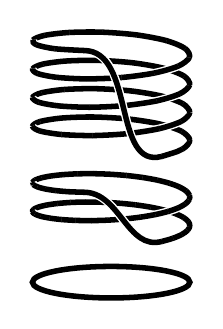
\begin{tikzpicture}[declare function={f(\x)=0.2*sin(\x)+\x/1000;},
 rubout/.style={/utils/exec=\tikzset{rubout/.cd,#1},
 decoration={show path construction,
      curveto code={
       \draw [white,line width=\pgfkeysvalueof{/tikz/rubout/line width}+2*\pgfkeysvalueof{/tikz/rubout/halo}] 
        (\tikzinputsegmentfirst) .. controls
        (\tikzinputsegmentsupporta) and (\tikzinputsegmentsupportb)  ..(\tikzinputsegmentlast); 
       \draw [line width=\pgfkeysvalueof{/tikz/rubout/line width},shorten <=-0.1pt,shorten >=-0.1pt] (\tikzinputsegmentfirst) .. controls
        (\tikzinputsegmentsupporta) and (\tikzinputsegmentsupportb) ..(\tikzinputsegmentlast);  
      }}},rubout/.cd,line width/.initial=2pt,halo/.initial=0.5pt]
 \draw[rubout={line width=2pt,halo=0.5pt},decorate] 
   plot[variable=\x,domain=-50:1330,samples=55,smooth] ({cos(\x)},{f(\x)}) to[out=0,in=195] cycle;
 \draw[rubout={line width=2pt,halo=0.5pt},decorate] 
   plot[variable=\x,domain=-1130:-470,samples=55,smooth] ({cos(\x)},{f(\x)}) to[out=0,in=195] cycle;

 \draw[line width=2pt] (0,-2) arc(-90:270:1cm and 0.2cm);
 % \draw[thick,-stealth]  (0,-0.4) -- (0,-1.4) node[midway,right]{$p$};
\end{tikzpicture}
\caption{Covering of the circle by a disjoint union of the four-to-one cover and the two-to-one cover.}
\label{fig:circle-cover-quadruple-double}
\end{figure}
\end{exmp}

The following diagram summarises the situation if $X$ is a `nice' space:
\begin{equation*}
    \begin{tikzcd}
        \catSheaf(X) \ar[r, "\simeq"] & \catLocalHomeomorphism_{/X} \\
        \catLocallyConstantSheaf(X) \ar[u, inclusion] \ar[r, "\simeq"'] & \catCoveringSpace_{/X} \ar[u, inclusion] \ar[r, "\simeq"'] & \homotopy[1](X,x)\catSet
    \end{tikzcd}
\end{equation*}
This diagram raises the question: what should there be in the top right spot?
Towards the end of the course, we will give a partial answer which goes by the name of \indexemph{exodromy}.

\chapter{Pullback and pushforward}

\remyquote{There is a risk you might learn something -- beware!}
\noindent
The goal of this lecture is to define a pair of adjoint functors
\begin{equation*}
  \begin{tikzcd}
    \catSheaf(Y) \ar[r, "f_*"'{name=rightadj}, shift right=2] &
    \catSheaf(X) \ar[l, "f^*"'{name=leftadj}, shift right=2]
    \ar[from=leftadj, to=rightadj, phantom, "\leftadj" rotate=-90]
  \end{tikzcd}
\end{equation*}
for a continuous map \(f\colon Y\to X\), called \indexemph{pullback} and \indexemph{pushforward}.
The strategy will be to first define these operations for presheaves, and then restrict to sheaves.
One of the functors will already send sheaves to sheaves, for the other we will postcompose the functor on the level of presheaves with sheafification.

\section{Pushforward}

A continuous map \(f\colon Y\to X\) induces a functor \(f\inv\colon\open(X)\to\open(Y)\) which sends an open set \(U\subseteq X\) to the open set \(f\inv(U)\subseteq Y\).
If \(U\subseteq V\subseteq X\) are open sets, then \(f\inv(U)\subseteq f\inv(V)\subseteq Y\), so this is indeed functorial.

\begin{defn}
The \indexdefnemph{pushforward} of a presheaf \(G\) on \(Y\) along \(f\) is the composite presheaf
\begin{equation*}
  f_*G \colon \open(X)\opp \xrightarrow{f\inv} \open(Y)\opp \xrightarrow{G} \catSet
\end{equation*}
on \(X\).
Explicitly, the value of the pushforward \(f_*G\) on an open \(U\subseteq X\) is \((f_*G)(U) = G(f\inv(U))\).
\end{defn}

The pushforward functor \(f_*\colon\catPresheaf(Y)\to\catPresheaf(X)\) is given by precomposition by the functor \(f\inv\colon\open(X)\opp\to\open(Y)\opp\), and so is indeed seen to be functorial.

\begin{lem}
If \(\mathcal G\) is a sheaf on \(Y\), then the pushforward \(f_*\mathcal G\) of \(\mathcal G\) along \(f\) is a sheaf on \(X\).
In particular, pushforward restricts to a functor \(f_*\colon\catSheaf(Y)\to\catSheaf(X)\) on the level of sheaves.
\end{lem}
\begin{proof}
Let \(U=\bigcup_{i\in I}U_i\) be an open cover in \(X\).
Then \(f\inv(U) = \bigcup_{i\in I}f\inv(U_i)\) is an open cover in \(Y\).
Applied to this cover, the sheaf condition for \(\mathcal G\) gives us an equaliser diagram
\begin{equation*}
  \begin{tikzcd}
    \mathcal G(f\inv(U)) \ar[r] & \prod_{i\in I}\mathcal G(f\inv(U_i)) \ar[r, shift left] \ar[r, shift right] & \prod_{i,j\in I}\mathcal G(f\inv(U_i\cap U_j))
  \end{tikzcd}
\end{equation*}
(where we have rewritten \(f\inv(U_i)\cap f\inv(U_j)=f\inv(U_i\cap U_j)\)), giving the sheaf condition for the pushforward \(f_*\mathcal G\).
\end{proof}

\section{Pullback}
\remyquote{Just sheafify the hell out of everything.}
\noindent
The \indexemph{pullback} of a sheaf on \(X\) along \(f\) should be a sheaf on \(Y\).
One way to approach the problem of constructing a presheaf on \(Y\) from a presheaf \(\mathcal F\) on \(X\), would be to try extending it along \(f\inv\) (and this is what we will attempt):
\begin{equation*}
  \begin{tikzcd}[column sep=tiny]
    \open(X)\opp \ar[rr, "\mathcal F"] \ar[rd, "f\inv"'] & & \catSet \\
    & \open(Y)\opp \ar[ru, dashed, "?"']
  \end{tikzcd}
\end{equation*}
In general, there might not be such an on-the-nose extension, but we can approximate an extension by considering extensions \emph{up to} a natural transformation.
There could be many such approximations, so we want to consider the `best possible approximation' in some suitable sense.

In category theory, the general problem of approximating an extension of a functor along another functor is studied using \indexemph{Kan extensions}; we refer to~\cite[Chapter~6]{riehlCategoryTheoryContext2016} for an introduction of Kan extensions, whose definition we actually do not need to know for our current purposes.
Here we will apply the general theory to our case to define the pullback of sheaves.\footnote{One can also construct and prove everything by hand, as was done in class, but this is rather tedious. We wish to illustrate with the following exposition that all the arguments will be completely formal.}

\begin{prop}\label{prop:pullback-Kan-extension}
Left Kan extensions\index{Kan extension} of presheaves on \(X\) (functors \(\open(X)\opp\to\catSet\)) along the functor \(f\inv\colon\open(X)\opp\to\open(Y)\opp\) exist, and assemble into a functor
\[\Lan*_{f\inv}\colon\catPresheaf(X)\to\catPresheaf(Y)\]
which is left adjoint to the \indexterm{pushforward} functor \(f_*\):
\begin{equation*}
  \begin{tikzcd}
    \catPresheaf(Y) \ar[r, "f_*"'{name=rightadj}, shift right=2] &
    \catPresheaf(X) \ar[l, "\Lan*_{f\inv}"'{name=leftadj}, shift right=2]
    \ar[from=leftadj, to=rightadj, phantom, "\leftadj" rotate=-90]
  \end{tikzcd}
\end{equation*}
Moreover, the left Kan extension along \(f\inv\) of a presheaf \(F\) on \(X\) is given on opens \(U\subseteq Y\) by
\begin{equation} \label{eq:left-Kan-extension-f-inv-colimit}
  \Lan_{f\inv} F(U) = \colim\displaylimits_{f\inv(W)\supseteq U}F(W)
\end{equation}
where \(W\) ranges over opens of \(X\) (more precisely, the colimit diagram is indexed by the full subcategory of \(\open(X)\) on those \(W\) such that \(f\inv(W)\supseteq U\), or equivalently \(W\supseteq f(U)\)).
\end{prop}
\begin{proof}
This is a special case of~\cite[Corollary~6.2.6]{riehlCategoryTheoryContext2016}; the only nontrivial step in applying the general result to this special case is recognising that the comma category \(f\inv\downarrow U\) for \(U\in\open(Y)\opp\) is the described index category, but this verification is elementary enough to be left to the reader.
\end{proof}

We would also like a description of what \(\Lan*_{f\inv}\) does on maps.
By a computation of the colimit in \cref{eq:left-Kan-extension-f-inv-colimit}, an element of \(\Lan*_{f\inv} F(U)\) is given by \([s]_W\) for some section \({s\in F(W)}\) for some \(W\supseteq f(U)\), where \([s]_W = [s']_{W'}\) if and only if there exists an open \(W''\subseteq W\cap W'\) containing \(f(U)\) such that \(s|_{W''} = s'|_{W''}\).
Unravelling the construction in \cite[Theorem~6.2.1]{riehlCategoryTheoryContext2016}, we see that the map induced by opens \(U\subseteq V\) in \(Y\) is given by
\[ \colim\displaylimits_{f\inv(W)\supseteq V}F(W) \to \colim\displaylimits_{f\inv(W)\supseteq U}F(W)\text{,} \quad [s]_W \mapsto [s]_W\text{.} \]

We may now define the pullback as follows:
\begin{defn}
The \emph{pullback}\index{pullback!of presheaves} \(f^{\circledast}F\) of a presheaf \(F\) on \(X\) along \(f\) is the left Kan extension of \(F\) along \(f\inv\).
The pullback functor is denoted \(f^{\circledast}\coloneq\Lan*_{f\inv}\colon\catPresheaf(X)\to\catPresheaf(Y)\).
\end{defn}

We have defined the pullback functor in such a way that it is left adjoint to the pushforward of presheaves.

We use the circled asterisk \(\circledast\) in the notation for the pullback of presheaves to distinguish it from the pullback of sheaves, which we will define momentarily, and for which we use a normal asterisk.\footnote{In class, we used the notation $f^{\textup{pre,*}}$ for $f^\circledast$, which we do not find very elegant.}
Unlike the pushforward, namely, the pullback of presheaves does not directly restrict to sheaves; that is to say, there are sheaves which are sent by \(f^{\circledast}\) to a presheaf which does not satisfy the sheaf condition, as witnessed by the following counterexample:

\begin{exmp}
Let $Y$ be the two-point space with the discrete topology, and let $X$ be the one-point space, with the unique map $f: Y \to X$. 
We can easily put a sheaf on $X$, for example by defining $\mathcal{F}(\emptyset) = *$ and $\mathcal{F}(X) = \{42, 43, 44\}$. 
The pullback in presheaves at any point $\{*\} \subset Y$ is $f^{\circledast}(\{*\}) = \colim_{f^{-1}(W) \supseteq *}\mathcal{F}(W) = \mathcal{F}(X) = \{42, 43, 44\}$. But the pullback in presheaves at $Y$ itself is also $\mathcal{F}(X) = \{42, 43, 44\}$. Check that the sheaf condition doesn't hold for the cover of $Y$ given by two opens, one containing precisely each point: the gluing condition on $\{42,43,44\} \times \{42, 43, 44\}$ is void because the points do not intersect.
\end{exmp}

\begin{defn}
The \emph{pullback}\index{pullback!of sheaves} \(f^*\mathcal F\) of a sheaf \(\mathcal F\) on \(X\) along a continuous map \(f\colon Y\to X\) is the sheaf
\[ f^*\mathcal F \coloneq (f^{\circledast}\mathcal F)^\sharp \]
on \(Y\), the sheafification of the presheaf pullback of \(\mathcal F\).
The pullback functor of sheaves is thus the composite
\[ f^* \colon \catSheaf(X) \hookrightarrow \catPresheaf(X) \xrightarrow{f^{\circledast}} \catPresheaf(Y) \xrightarrow{(-)^\sharp} \catSheaf(Y)\text{.} \]
\end{defn}

Note that the definition of the pullback also makes sense for presheaves; we also denote the functor \(\catPresheaf(X)\to\catSheaf(Y)\) sending a presheaf \(F\) to the pullback \(f^*F = (f^\circledast)^\sharp\) by \(f^*\).

\begin{prop}\label{lem:pushforward-pullback-adjunction-sheaves}
Pushforward and pullback of sheaves along \(f\) define an adjunction
\begin{equation*}
  \begin{tikzcd}
    \catSheaf(Y) \ar[r, "f_*"'{name=rightadj}, shift right=2] &
    \catSheaf(X) \ar[l, "f^*"'{name=leftadj}, shift right=2]
    \ar[from=leftadj, to=rightadj, phantom, "\leftadj" rotate=-90]
  \end{tikzcd}
\end{equation*}
\end{prop}
\begin{proof}
Compose the adjunctions
\begin{equation*}
  \begin{tikzcd}
    \catSheaf(Y) \ar[r, ""'{name=rightadj1}, inclusion, shift right=2] \ar[rrd, "f_*"', bend right=15] &
    \catPresheaf(Y) \ar[l, "(-)^\sharp"'{name=leftadj1}, shift right=2] \ar[r, "f_*"'{name=rightadj2}, shift right=2] &
    \catPresheaf(X) \ar[l, "f^{\circledast}"'{name=leftadj2}, shift right=2] \ar[ll, "f^*"', bend right=15, shift right=5] \\
    & & \catSheaf(X) \ar[u, inclusion]
    \ar[from=leftadj1, to=rightadj1, phantom, "\leftadj" rotate=-90]
    \ar[from=leftadj2, to=rightadj2, phantom, "\leftadj" rotate=-90]
  \end{tikzcd}
\end{equation*}
of \cref{cor:sheafification-left-adjoint-to-inclusion} and \cref{prop:pullback-Kan-extension}.
\end{proof}

Between the sets $\Hom[\catSheaf(Y)](f^*\mathcal F,\mathcal G)$ and $\Hom[\catSheaf(X)](\mathcal F,f_*\mathcal G)$ which are naturally isomorphic by the adjunction, there is also an `intermediate' set of maps, called \emph{$f$-maps}; see~\cite[\href{https://stacks.math.columbia.edu/tag/008K}{Lemma 008K}]{stacks-project}.

From the fact that the pushforward already sends sheaves to sheaves (so its definition `doesn't need sheafification'), we obtain the following corollary, showing that pulling back the sheafification of a presheaf is the same as pulling back the presheaf.

\begin{cor}\label{cor:pullback-sheafification}
Let \(f\colon Y\hookrightarrow X\) be a continuous map.
Then the functors
\[ \catPresheaf(X) \xrightarrow{f^*} \catSheaf(Y) \qquad \text{and} \qquad \catPresheaf(X) \xrightarrow{(-)^\sharp} \catSheaf(X) \xrightarrow{f^*} \catSheaf(Y) \]
are naturally isomorphic.
\end{cor}
\begin{proof}
  % and write \(\iota\colon\catSheaf(X)\hookrightarrow\catPresheaf(X)\) for the full subcategory inclusion
By definition, the former functor is the composite
\begin{equation*}
  \begin{tikzcd}
    \catPresheaf(X) \ar[r, "f^\circledast"{name=leftadj1}, shift left=2] &
    \catPresheaf(*) \ar[l, "f_*"{name=rightadj1}, shift left=2] \ar[r, "(-)^\sharp"{name=leftadj2}, shift left=2] &
    \catSheaf(*) \ar[l, ""{name=rightadj2}, shift left=2, inclusion]
    \ar[from=leftadj1, to=rightadj1, phantom, "\leftadj" rotate=-90]
    \ar[from=leftadj2, to=rightadj2, phantom, "\leftadj" rotate=-90]
  \end{tikzcd}
\end{equation*}
of the presheaf pullback along \(f\) and sheafification, which have right adjoints given by respectively the pushforward along \(f\) and the full subcategory inclusion by \cref{prop:pullback-Kan-extension} and \cref{cor:sheafification-left-adjoint-to-inclusion}.
The latter functor has a right adjoint
\begin{equation*}
  \begin{tikzcd}
    \catPresheaf(X) \ar[r, "(-)^\sharp"{name=leftadj1}, shift left=2] &
    \catSheaf(X) \ar[l, ""{name=rightadj1}, shift left=2, inclusion] \ar[r, "f^*"{name=leftadj2}, shift left=2] &
    \catSheaf(*) \ar[l, "f_*"{name=rightadj2}, shift left=2]
    \ar[from=leftadj1, to=rightadj1, phantom, "\leftadj" rotate=-90]
    \ar[from=leftadj2, to=rightadj2, phantom, "\leftadj" rotate=-90]
  \end{tikzcd}
\end{equation*}
given by pushforward along \(f\) followed by the full subcategory inclusion by \cref{cor:sheafification-left-adjoint-to-inclusion} and \cref{lem:pushforward-pullback-adjunction-sheaves}.
These two right adjoint are equal by definition, so we find the required natural isomorphism.
\end{proof}

The following corollary roughly says that pushforward and pullback are `functorial in the map' (respectively co- and contravariantly).\footnote{This statement can probably be made precise in terms of \(2\)-categories.}

\begin{cor}
For any space \(X\), we have \((\id_X)_*=\id_{\catSheaf(X)}\cong(\id_X)^*\), and for any maps \(f\colon Z\to Y\) and \(g\colon Y\to X\) we have \((gf)_*=g_*f_*\colon\catSheaf(Z)\to\catSheaf(X)\) and \((gf)^*\cong f^*g^*\colon\catSheaf(X)\to\catSheaf(Z)\).
\end{cor}
Note that the identities for the pushforward hold on-the-nose, whereas we only prove the identities for the pullback up to natural isomorphism.
\begin{proof}
The identities for the pushforward follow directly from the definition since \((gf)\inv(U)=f\inv(g\inv(U))\).
The identities for the pullback follow from those for the pushforward and the adjunction of \cref{lem:pushforward-pullback-adjunction-sheaves}: we have adjunctions \((gf)^*\leftadj(gf)_*\) and \(f^*g^*\leftadj g_*f_*\) and the right adjoints in these adjunctions are equal.
\end{proof}

\section{Stalks, germs, skyscrapers}

\begin{defn}\label{defn:stalk}
Let $i_x\colon \{x\} \hookrightarrow X$ be the inclusion of a point in a space.
Then $i_x^* \mathcal{F}$ is the \indexdefnemph{stalk} $\mathcal{F}_x$ of $\mathcal{F}$ at $x$; this is a sheaf on a point, so equivalently a set by \cref{exmp:sheaf-on-point-set} (the value of the sheaf on the whole space).
Unravelling definitions, we have \[
    \mathcal{F}_x = \colim_{U \ni x} \mathcal{F}(U)\text{.}
\]
An element of the stalk at $x$ is represented by a \indexdefnemph{germ} $[s]_U$ for $U \ni x$ and $s \in \mathcal{F}(U)$, where \([s]_U = [t]_V\) if and only if there exists an open neighbourhood \(W\subseteq U\cap V\) of \(x\) such that \(s|_W=t|_W\).
\end{defn}
Note that the stalk $\mathcal{F}_x$ is the fibre of $\etalespace(X) \to X$ over $x$. 

\begin{rmk}
\Cref{cor:pullback-sheafification} tells us that we can compute the stalks of the sheafification of a presheaf by computing the stalks of the presheaf itself.
\end{rmk}

\begin{exmp}[orientation sheaf of a \indexterm{manifold}]
Let \(M\) be an \(n\)-dimensional topological manifold, by which we mean a Hausdorff space that is locally homeomorphic to \(\bb R^n\) (i.e., every point of \(M\) admits a neighbourhood homeomorphic to \(\bb R^n\)).
For a subset \(K\subseteq M\), we write \[H_k(M\mid K;R) \coloneq H_k(M,M\setminus K;R)\] for the \(k\)th homology of \(M\) relative to \(M\setminus K\) with coefficients in a commutative ring \(R\).

A \emph{local \(R\)-orientation} at a point \(x\in M\) is a generator \(\mu_x\) of \(H_n(M\mid x;R)\cong R\) (note that we take homology in degree \(n\), the dimension of the manifold \(M\)).
That \(H_n(M\mid x;R)\) is isomorphic to \(R\) (as \(R\)-modules) follows from excision; choosing a generator corresponds exactly to choosing such an isomorphism.
An \emph{\(R\)-orientation}\index{manifold!orientation} of \(M\) is a family of local orientations \((\mu_x)_{x\in M}\) with the property that every point \(y\in M\) admits a compact neighbourhood \(K\) and an element \(\mu_K\in H_n(M\mid K;R)\) such that \(\mu_K\) restricts to \(\mu_x\) for any \(x\in K\) under the map \(H_n(M\mid K;R)\to H_n(M\mid x;R)\) induced by the inclusion \(M\setminus K\to M\setminus\{x\}\).

There is a sheaf \(\mathcal O_M\) of \(R\)-modules, the \emph{orientation sheaf}\index{manifold!orientation sheaf} of \(M\), defined by
\[\mathcal O_M(U)\coloneq H_n(M\mid U;R)\]
for \(U\subseteq M\) open.
The restriction map for opens \(U\subseteq V\subseteq M\) is induced by the inclusion of pairs \((M,M\setminus V)\hookrightarrow(M,M\setminus U)\).
The stalk of the orientation sheaf \(\mathcal O_M\) at \(x\in M\) is the \(R\)-module \(H_n(M\mid x;R)\).
\end{exmp}

\begin{rmk}
One can show (as a generalisation of an exercise in Homework 3) that the étalé space of the pullback can be obtained as a \indexterm{fibre product}. More precisely, given $f\colon Y \to X$, the diagram 
\[\begin{tikzcd}
	{\etalespace(f^*\mathcal{F})} & {\etalespace(\mathcal{F})} \\
	Y & X
	\arrow[from=1-1, to=2-1]
	\arrow[from=2-1, to=2-2]
	\arrow[from=1-2, to=2-2]
	\arrow[from=1-1, to=1-2]
	\arrow[pullback, from=1-1, to=2-2]
\end{tikzcd}\]
is a pullback square. 
This is used in \todo{Add cite MacLane Moerdijk} to define $f^*$. 
\end{rmk}


Given a map $\alpha\colon \mathcal{F} \to \mathcal{G}$ between sheaves on a space $X$ and a point $x \in X$, there is an induced map on stalks $\alpha_x\colon \mathcal{F}_x \to \mathcal{G}_x$, because $\mathcal{G}_x$ is a cocone over
\[\setpred{\mathcal{F}(U)}{U \in \open(X),x \in U}\text{,}\]
of which $\mathcal{F}_x$ is a colimit. 

\begin{lem}\label{lem:stalkwise-check-isomorphism}
    Let $\alpha\colon \mathcal{F} \to \mathcal{G}$ be a map in $\catSheaf(X)$. 
    Then $\alpha$ is an isomorphism of sheaves if and only if $\alpha_x\colon \mathcal{F}_x \to \mathcal{G}_x$ is a bijection for all $x \in X$. 
\end{lem}
\begin{proof}
    The map $\etalespace(\alpha)\colon \etalespace(\mathcal{F}) \to \etalespace(\mathcal{G})$ is a local homeomorphism over $X$, because the maps $\etalespace(\mathcal{F}) \to X$ and $\etalespace(\mathcal{G}) \to X$ are local homeomorphisms. In particular, $\etalespace(\alpha)$ is an open map. So it is invertible if and only if it is a bijection. Check that this is equivalent to requiring that the map on the fibres over $x$ is a bijection for all $x \in X$. Since the stalks $\mathcal{F}_x$ and $\mathcal{G}_x$ are exactly these fibres, we are done. 
\end{proof}

\begin{defn}
    Let $\{x\} \to X$ be the inclusion of a point $x \in X$. Let $S \in \catSet$. The \indexemph{skyscraper sheaf} at $x$ with value $S$ is $i_{x,*}\underline{S}$, the pushforward of the constant sheaf. We denote it $i_{*, S}$.
\end{defn}

\begin{exmp}
    Let $\{0\} \to \bb R$ be the inclusion of zero into the real numbers. Let $S = \{a,b\}$. Then the skyscraper sheaf is 
    \[
        i_{*,S}(U) = S(U \cap 0) =     \begin{cases}
        \{a,b\} & \text{if } 0 \in U\\
        * & \text{if } x \notin U.
    \end{cases}
    \]
    In Homework 2, we saw that the étalé space of this sheaf is the line with two origins. 
\end{exmp}
\subfile{Lectures/Lecture 6}
\subfile{Lectures/Lecture 7}
\subfile{Lectures/Lecture 8}
\chapter{Monomorphisms and epimorphisms, chain complexes, exact sequences}\label{lecture:9}

In the last lecture, we defined abelian categories as \(\catAbelianGroup\)-enriched categories \(\cat A\) with finite limits and colimits in which the first isomorphism theorem holds (the natural map \(\coim f\to\im f\) is an isomorphism for all \(f\colon A\to B\) in \(\cat A\)).
We also showed that the category \(\catAbelianPresheaf(X)\) of abelian presheaves on a space \(X\) is an abelian category.

Today we will show that also the category \(\catAbelianSheaf(X)\) of abelian sheaves on \(X\) is an abelian category, and we will give a description of monomorphisms and epimorphisms.

\section{Abelian category of abelian sheaves}

\begin{lem}\label{lem:pullback-preserves-colimits-and-finite-limits}
Let \(f\colon Y\to X\) be a continuous map.
Then the pullback functors \(f^*\colon\catSheaf(X)\to\catSheaf(Y)\) and \(f^*\colon\catAbelianSheaf(X)\to\catAbelianSheaf(Y)\) preserve finite limits and all colimits.
\end{lem}
\begin{proof}
Since the pullback functor \(f^*\) is left adjoint to the pushforward functor \(f_*\) (\cref{lem:pushforward-pullback-adjunction-sheaves}), it preserves colimits.

For finite limits, there are two methods:
\begin{enumerate}
\item Use that \(f^*\) is given by
  \[\catLocalHomeomorphism_{/X}\to\catLocalHomeomorphism_{/Y}\text{,} \quad (Z\to X) \mapsto \bigl(Z\pullback{X}Y\to Y\bigr)\text{,} \]
  which preserves finite limits, and finite limits in \(\catLocalHomeomorphism_{/-}\) are computed as in \(\catTopologicalSpace_{/-}\).\footnote{This does not hold for all limits; it fails for instance for infinite products, already when \(X\) is a point.}
\item Use that
  \[(f^\circledast\mathcal F)(U) = \colim_{f(U)\subseteq V}\mathcal F(V) \]
  is a filtered colimit, and filtered colimits in \(\catSet\) and \(\catAbelianGroup\) commute with finite limits (Additional exercise~9.1).
  Check that sheafification preserves finite limits (Homework~5).
  \qedhere
\end{enumerate}
\end{proof}

\begin{prop}
If \(X\) is a topological space, then the category \(\catAbelianSheaf(X)\) of abelian sheaves on \(X\) is an abelian category.
\end{prop}
\begin{proof}
Being a full subcategory of the abelian category \(\catAbelianPresheaf(X)\), the category \(\catAbelianSheaf(X)\) is pre-additive, and we have already shown in \cref{thm:limits-colimits-sheaves} that it has all limits and colimits.

It remains to check that the first isomorphism theorem holds in \(\catAbelianSheaf(X)\).
Let \(f\colon\mathcal F\To\mathcal G\) be a map in \(\catAbelianSheaf(X)\).
We can factor \(f\) as
\begin{equation}\label{eq:factorisation-coimage-image}
  \mathcal F \To \coim f \To \im f \To \mathcal G\text{.}
\end{equation}
By \cref{lem:pullback-preserves-colimits-and-finite-limits}, the formation of the kernel, cokernel, image and coimage commutes with the stalk functor \(i_x^*\) for all \(i_x\colon\{x\}\to X\) (see \cref{defn:stalk}).
So \cref{eq:factorisation-coimage-image} induces the factorisation
\[ \mathcal F_x \to (\coim f)_x = \coim f_x \to (\im f)_x = \im f_x \to \mathcal G_x \]
of the map \(f_x\) induced on stalks.
The map \(\coim f_x\to\im f_x\) is an isomorphism since \(\catAbelianGroup\) is an abelian category.
Since this holds for all stalks, the map \(\coim f\to\im f\) is also an isomorphism by \cref{lem:stalkwise-check-isomorphism}.
\end{proof}

\section{Monomorphisms and epimorphisms}

\begin{lem}
Let \(\cat A\) be an abelian category and \(f\colon A\to B\) a map in \(\cat A\).
Then:
\begin{enumerate}
\item \(f\) is monic if and only if \(\ker f = 0\);
\item \(f\) is epic if and only if \(\coker f = 0\).
\end{enumerate}
\end{lem}

The recipe of the proof is: Yoneda + the same statement in \(\catAbelianGroup\).

\begin{proof}
\begin{enumerate}
\item
  By definition, \(\ker f\) represents \(\ker(\Hom[\cat A](-,A)\To\Hom[\cat A](-,B))\).
  So \(\ker f = 0\) if and only if \(\Hom[\cat A](-,A)\To\Hom[\cat A](-,B)\) is an injective map of presheaves, that is, \(f\colon A\to B\) is monic.
\item Follows dually. \qedhere
\end{enumerate}
\end{proof}

For sheaves, let's make it quite concrete.

\begin{lem}\label{lem:monomorphisms-sheaves}
Let \(f\colon\mathcal F\To\mathcal G\) be a map in \(\catSheaf(X)\) (resp.~\(\catAbelianSheaf(X)\)).
Then the following are equivalent:
\begin{enumerate}
\item\label{lem:monomorphisms-sheaves:monic-sheaves} \(f\) is monic (in \(\catSheaf(X)\) resp.~\(\catAbelianSheaf(X)\));
\item\label{lem:monomorphisms-sheaves:monic-presheaves} \(f\) is monic in \(\catPresheaf(X)\) (resp.~\(\catAbelianPresheaf(X)\));
\item\label{lem:monomorphisms-sheaves:injective-open} \(f_U\) is injective for all open subsets \(U\subseteq X\);
\item\label{lem:monomorphisms-sheaves:injective-stalk} \(f_x\) is injective for all points \(x\in X\);
\item\label{lem:monomorphisms-sheaves:injective-etale-space} \(\etalespace(f)\to X\) is injective.
\end{enumerate}
\end{lem}
\begin{proof}
By Additional exercise~7.3, we know that \(f\) is monic if and only if the diagram
\begin{equation*}
  \begin{tikzcd}[arrows=Rightarrow]
    \mathcal F \ar[r, "\id"] \ar[d, "\id"'] & \mathcal F \ar[d, "f"] \\
    \mathcal F \ar[r, "f"'] & \mathcal G
  \end{tikzcd}
\end{equation*}
is a pullback square.
So the equivalence of \cref{lem:monomorphisms-sheaves:monic-sheaves} and \cref{lem:monomorphisms-sheaves:monic-presheaves} follows since the inclusion \(\catSheaf(X)\hookrightarrow\catPresheaf(X)\) (resp.~\(\catAbelianSheaf(X)\hookrightarrow\catAbelianPresheaf(X)\)) creates limits (\cref{thm:limits-colimits-sheaves}), and the equivalence of \cref{lem:monomorphisms-sheaves:monic-presheaves} and \cref{lem:monomorphisms-sheaves:injective-open} since limits in \(\catPresheaf(X)\) (resp.~\(\catAbelianPresheaf(X)\)) are computed objectwise.

The functors
\begin{equation*}
  \begin{tikzcd}
    \catSheaf(X) \ar[r, "\simeq"] & \catLocalHomeomorphism_{/X} \ar[r, inclusion] & \catTopologicalSpace_{/X} \ar[r, inclusion] & \catSet_{/X}
  \end{tikzcd}
\end{equation*}
(and the corresponding functors for abelian sheaves) create fibre products, so they preserve and reflect monomorphisms.
Since monomorphisms in \(\catSet_{/X}\) (resp.~\(\catAbelianGroup(\catSet_{/X})\)) are injective maps, this proves that \cref{lem:monomorphisms-sheaves:monic-sheaves} is equivalent to \cref{lem:monomorphisms-sheaves:injective-etale-space}.

Finally, \cref{lem:monomorphisms-sheaves:injective-stalk} is equivalent to \cref{lem:monomorphisms-sheaves:injective-etale-space} since the fibres of \(\etalespace(\mathcal F)\to\etalespace(\mathcal G)\) over \(x\in X\) are the stalks \(f_x\).
\end{proof}

The epimorphisms of sheaves are more subtle.
Although the epimorphisms of presheaves are just objectwise epimorphisms (characterisation~\cref{lem:monomorphisms-sheaves:injective-open} of the last lemma), this is not true for epimorphisms of sheaves.
This is perhaps to be expected: monomorphisms are related to limits (as discussed in the last proof), and the forgetful functor from sheaves to presheaves creates limits, but epimorphisms are related to colimits (in a dual way, made precise in the following proof), whose relation to colimits of presheaves is not so straightforward.

\begin{lem}\label{lem:epimorphisms-sheaves}
Let \(f\colon\mathcal F\To\mathcal G\) be a map in \(\catSheaf(X)\) (resp.~\(\catAbelianSheaf(X)\)).
Then the following are equivalent:
\begin{enumerate}
\item\label{lem:epimorphisms-sheaves:epic-sheaves} \(f\) is epic (in \(\catSheaf(X)\) resp.~\(\catAbelianSheaf(X)\));
\item\label{lem:epimorphisms-sheaves:locally-lift-section} for every open subset \(U\subseteq X\) and every section \(t\in\mathcal G(U)\), there exists an open cover \(U=\bigcup_{i\in I}U_i\) and sections \(s_i\in\mathcal F(U_i)\) such that \(f(s_i) = t|_{U_i}\);
\item\label{lem:epimorphisms-sheaves:surjective-stalk} \(f_x\) is surjective for all points \(x\in X\);
\item\label{lem:epimorphisms-sheaves:surjective-etale-space} \(\etalespace(f)\to X\) is surjective.
\end{enumerate}
In \(\catAbelianSheaf(X)\), these statements are also equivalent to:
\begin{enumerate}[resume]
\item\label{lem:epimorphisms-sheaves:surjective-etale-space} the sheafification of the presheaf cokernel is zero.
\end{enumerate}
\end{lem}
\begin{proof}
Again, \(f\) is epic if and only if the diagram
\begin{equation*}
  \begin{tikzcd}[arrows=Rightarrow]
    \mathcal F \ar[r, "f"] \ar[d, "f"'] & \mathcal G \ar[d, "\id"] \\
    \mathcal G \ar[r, "\id"'] & \mathcal G
  \end{tikzcd}
\end{equation*}
is a pushout square.
If this holds, it holds for all stalks \(f_x\colon\mathcal F_x\to\mathcal G_x\) since \(i_x^*\) preserves colimits by \cref{lem:pullback-preserves-colimits-and-finite-limits}.
This proves that \cref{lem:epimorphisms-sheaves:epic-sheaves} implies \cref{lem:epimorphisms-sheaves:surjective-stalk}, and the equivalence of \cref{lem:epimorphisms-sheaves:surjective-stalk} and \cref{lem:epimorphisms-sheaves:surjective-etale-space} is clear since surjectivity in \(\catTopologicalSpace_{/X}\) is checked fibrewise.
Conversely, that \cref{lem:epimorphisms-sheaves:surjective-etale-space} implies \cref{lem:epimorphisms-sheaves:epic-sheaves} follows from the equivalence \(\catSheaf(X)\simeq\catLocalHomeomorphism_{/X}\) (resp.~\(\catAbelianSheaf(X)\simeq\catAbelianGroup(\catLocalHomeomorphism_{/X})\)) since a surjection in \(\catLocalHomeomorphism_{/X}\) is surely an epimorphism\footnote{This holds in any \emph{concrete category} \(\cat C\), a category with a faithful functor \(\cat C\to\catSet\), since faithful functors reflect epimorphisms.}.

The equivalence of \cref{lem:epimorphisms-sheaves:locally-lift-section} and \cref{lem:epimorphisms-sheaves:surjective-stalk} is an unwinding of the definitions.
Statement~\cref{lem:epimorphisms-sheaves:locally-lift-section} means that for all \(x\in U\) and all \(t\in\mathcal G(U)\) there exists \(x\in U'\subseteq U\) and \(s\in\mathcal F(U)\) such that \(f(s) = t|_{U'}\), which is \cref{lem:epimorphisms-sheaves:surjective-stalk}.

In the abelian case, the equivalence of \cref{lem:epimorphisms-sheaves:epic-sheaves} and \cref{lem:epimorphisms-sheaves:surjective-etale-space} follows from the construction of the sheaf cokernel as the sheafification of the presheaf cokernel.
\end{proof}

\begin{defn}
A map in an abelian category is called \emph{injective} if it is a monomorphism and \emph{surjective} if it is an epimorphism.
\end{defn}

\todo{warning sign?}

\begin{rmk}
If \(f\colon\mathcal F\To\mathcal G\) is a surjective map of abelian sheaves, then the component \(\mathcal F(U)\to\mathcal G(U)\) need not be surjective.

In Homework~3, we constructed a surjection \(f\colon\mathcal F\To i_*i^*\mathcal F\) for any closed inclusion \(i\colon Z\hookrightarrow X\) and any abelian sheaf \(\mathcal F\) on \(X\).
Take \(X=\bb R\), \(Z = \{0,1\}\subseteq\bb R\) and \(F=\constSheaf{\bb Z}\).
Then \(i^*\mathcal F = \constSheaf{\bb Z}\) (pullbacks of constant sheaves are constant sheaves) and \(\constSheaf{\bb Z}\to i_*\constSheaf{\bb Z}\) is surjective.
But plugging in \(\bb R\) gives the map
\[\constSheaf{\bb Z}(\bb R) = \bb Z \to (i_*\constSheaf{\bb Z})(\bb R) = \constSheaf{\bb Z}(\bb R\cap\{0,1\}) = \bb Z\oplus\bb Z\text{,} \quad a \mapsto (a,a)\text{.} \]
which is not surjective.
However, any \((a,b)\in\bb Z\oplus\bb Z\) can be lifted: the open sets \(U_0\coloneq(-\infty,1)\), \(U_1\coloneq(0,\infty)\) cover \(\bb R\) and \((a,b)\) locally lifts to \(s_0\coloneq a\) and \(s_1\coloneq b\), but they do not glue.
\todo{Picture}
(Another example is on Homework~5.)
\end{rmk}

\section{Exact sequences}

\begin{lem}\label{lem:mono-epi-abelian-category}
Let \(\cat A\) be an abelian category and \(f\colon A\to B\) a map in \(\cat A\).
Then:
\begin{enumerate}
\item\label{lem:mono-epi-abelian-category:i} The map \(\ker f\to A\) (resp.~\(B\to\coker f\)) is monic (resp.~epic), and an isomorphism if \(f=0\).
\item\label{lem:mono-epi-abelian-category:ii} The map \(\im f\to B\) (resp.~\(A\to\coim f\)) is monic (resp.~epic), and an isomorphism if \(f\) is epic (resp.~monic).
\item\label{lem:mono-epi-abelian-category:iii} \(\ker f\) is canonically isomorphic to \(\ker(A\to\coim f)\), and \(\coker f\) is canonically isomorphic to \(\coker(\im f\to B)\).
\item\label{lem:mono-epi-abelian-category:iv} If \(f\) is monic (resp.~epic), then \(A\cong\ker(B\to\coker f)\) (resp.~\(B\cong\coker(\ker f\to A)\)).
  (In particular, any monomorphism (resp.~epimorphism) is an equaliser (resp.~coequaliser), hence a \emph{regular} monomorphism (resp.~epimorphism).)
\item\label{lem:mono-epi-abelian-category:v} If \(f\) is both monic and epic, then it is an isomorphism.
  (\(\cat A\) is a \emph{balanced} category.)
\end{enumerate}
\end{lem}
\begin{proof}
\begin{enumerate}
\item
  The universal property of \(\ker f\) is
  \[\Hom[\cat A](C,\ker f) \cong \setpred{\phi\in\Hom[\cat A](C,A)}{f\phi = 0}\text{,} \]
  so \(\Hom[\cat A](C,\ker f)\to\Hom[\cat A](C,A)\) is injective for all \(C\), hence \(\ker f\to A\) is monic.
  If \(f=0\), the condition \(f\phi=0\) on \(\phi\) is vacuous, so \(\Hom[\cat A](C,\ker f)\cong\Hom[\cat A](C,A)\).
  The statements about \(B\to\coker f\) follow dually.
\item
  Apply \cref{lem:mono-epi-abelian-category:i} to \(B\to\coker f\) (resp.~\(\ker f\to A\)), which we saw is zero if \(f\) is epic (resp.~monic).
\item
  We have a factorisation
  \begin{equation*}
    \begin{tikzcd}[column sep=scriptsize]
      A \ar[r, "\pi", epi] & \coim f \ar[r, iso'] & \im f \ar[r, mono] & B
    \end{tikzcd}
  \end{equation*}
  of \(f\) by \cref{lem:mono-epi-abelian-category:ii}, so the map \(\coim f\to B\) is monic.
  Then for any \(\phi\colon C\to A\), the composition \(\pi\phi=0\) if and only if \(f\phi=0\), so \(\ker\pi=\ker f\).
  The other statement follows dually.
\item
  If \(f\) is monic, then \(A\cong\coim f\cong\im f\) by \cref{lem:mono-epi-abelian-category:ii}.
  The other statement follows dually.
\item
  By \cref{lem:mono-epi-abelian-category:ii}, all maps
  \begin{equation*}
    \begin{tikzcd}[column sep=scriptsize]
      A \ar[r] & \coim f \ar[r, iso'] & \im f \ar[r] & B
    \end{tikzcd}
  \end{equation*}
  are isomorphisms.
  \qedhere
\end{enumerate}
\end{proof}

\begin{defn}
A \emph{cochain complex} in an additive category \(\cat C\) is a diagram
\begin{equation*}
  \begin{tikzcd}
    \ldots \ar[r] & C^{i-1} \ar[r, "d^{i-1}"] & C^i \ar[r, "d^i"] & C^{i+1} \ar[r] & \ldots
  \end{tikzcd}
\end{equation*}
in \(\cat C\) such that \(d^{i+1}d^i=0\) for all \(i\in\bb Z\).
(If it is only defined on a subset \(I\subseteq\bb Z\), we set \(C^i\coloneq 0\) for \(i\notin I\).)

A cochain complex \(C^\bullet\) is \emph{exact} at \(C^i\) if the canonical map \(\im d^{i-1}\to\ker d^i\) is an isomorphism.

A \emph{short exact sequence} is an exact complex \(0\to A\to B\to C\to 0\).

A \emph{cochain map} \(f^\bullet\colon C^\bullet\to D^\bullet\) of cochain complexes is a natural transformation in \(\catFunctor(\bb Z,\cat C)\):
\begin{equation*}
  \begin{tikzcd}
    \ldots \ar[r] & C^{i-1} \ar[r, "d^{i-1}"] \ar[d, "f^{i-1}"'] & C^i \ar[r, "d^i"] \ar[d, "f^i"] & C^{i+1} \ar[r] \ar[d, "f^{i+1}"] & \ldots \\
    \ldots \ar[r] & D^{i-1} \ar[r, "d^{i-1}"'] & D^i \ar[r, "d^i"'] & D^{i+1} \ar[r] & \ldots
  \end{tikzcd}
\end{equation*}
\end{defn}

The following lemma shows that our previous \emph{ad hoc} notion of exactness of \cref{defn:short-exact-sequence-sheaves} agrees with the categorical notion.

\begin{lem}
Let \(\mathcal F^\bullet\) be a cochain complex in \(\catAbelianSheaf(X)\).
Then \(\mathcal F^\bullet\) is exact at \(\mathcal F^i\) if and only if \(\mathcal F^\bullet_x\) is exact at \(\mathcal F^i_x\) is exact for all \(x\in X\).
\end{lem}

\begin{proof}
We saw in \cref{lem:pullback-preserves-colimits-and-finite-limits} that \(i_x^*\colon\catAbelianSheaf(X)\to\catAbelianGroup\) preserves all finite limits and colimits, so in particular the kernel, cokernel, image and coimage.
Thus, we conclude since \(\im d^{i-1}\To\ker d^i\) is an isomorphism if and only if \((\im d^{i-1})_x\to(\ker d^i)_x\) is an isomorphism for all \(x\in X\) by \cref{lem:stalkwise-check-isomorphism}.
\end{proof}

%%% Local Variables:
%%% mode: latex
%%% TeX-master: "../main"
%%% End:

\chapter{Exact functors, diagram lemmas}

\section{Exact functors}
\remyquote{For the five lemma, if you look at three different sources, you'll get three different lemmas. That's the three lemma.}
\noindent
\begin{defn}
Let \(\cat C\) and \(\cat D\) be categories and assume \(\cat C\) has finite limits (resp.~finite colimits).
Then a functor \(F\colon\cat C\to\cat D\) is \emph{left exact} (resp.~\emph{right exact}) if it preserves finite limits (resp.~finite colimits).
The functor \(F\) is \emph{exact} if it is both left and right exact.
\end{defn}

The goal of today is to show that this definition agrees with the definition in terms of short exact sequences.

\begin{exmp}
\begin{itemize}
\item 
  If \(F\) has a right adjoint, then it is right exact.
  If \(F\) \emph{is} a right adjoint (so \emph{has} a left adjoint), then it is left exact.
\item
  We proved that \(f^*\colon\catSheaf(X)\to\catSheaf(Y)\) for \(f\colon Y\to X\) is exact in \cref{lem:pullback-preserves-colimits-and-finite-limits}.
\item
  On Homework~5, we show that sheafification \((-)^\sharp\colon\catPresheaf(X)\to\catSheaf(X)\) (or for abelian sheaves) is exact.
\item
  The forgetful functor \(\catTopologicalSpace\to\catSet\) is exact since it has adjoints on both sides, equipping a set with the discrete or indiscrete topology.
\item
  The forgetful functor \(\catAbelianGroup\to\catSet\) is left exact, but not right exact since \(A\oplus B\neq A\cotimes B\).
\end{itemize}
\end{exmp}

\begin{defn}
Let \(\cat C\) and \(\cat D\) be pre-additive categories.
Then a functor \(F\colon\cat C\to\cat D\) is \emph{additive} if the maps \(\Hom[\cat C](X,Y)\to\Hom[\cat D](FX,FY)\) are group homomorphisms.
\end{defn}

Most functors between abelian categories in nature are additive.

\begin{exmp}
\begin{itemize}
\item
  If \(\cat C\) is a pre-additive category with an object \(X\), then the representable functor \(\Hom[\cat C](-,X)\colon\cat C\opp\to\catAbelianGroup\) is additive: the map
  \[ \Hom[\cat C](Y,Z) \to \Hom[\catAbelianGroup](\Hom[\cat C](Z,X),\Hom[\cat C](Y,X))\text{,} \quad f \mapsto (g\mapsto g\circ f) \]
  is a group homomorphism since composition in a pre-additive category is bilinear.
  Likewise, the corepresentable functor \(\Hom[\cat C](X,-)\colon\cat C\to\catAbelianGroup\) is also additive.
\item
  The free--forgetful adjunction between abelian groups and sets gives a monad (in particular an endofunctor) on \(\catAbelianGroup\), which is not additive: it sends the zero object to \(\bb Z\) and the identity of \(0\), which is also the zero map, must be sent to the identity of \(\bb Z\) by functoriality and to the zero map of \(\bb Z\) by additivity.
\end{itemize}
\end{exmp}

The problem in the last non-example was that the functor did not preserve the zero object.

\begin{lem}\label{lem:characterisation-additive-functor}
Let \(\cat C\) and \(\cat D\) be additive categories and \(F\colon\cat C\to\cat D\) a functor.
Then the following are equivalent:
\begin{enumerate}
\item\label{lem:characterisation-additive-functor:additive} \(F\) is additive;
\item\label{lem:characterisation-additive-functor:products} \(F\) preserves finite products;
\item\label{lem:characterisation-additive-functor:coproducts} \(F\) preserves finite coproducts;
\item\label{lem:characterisation-additive-functor:biproducts} \(F\) preserves binary biproducts.
\end{enumerate}
\end{lem}
\begin{proof}
Note that \cref{lem:characterisation-additive-functor:biproducts} implies that \(F\) preserves the zero object: the biproduct of the zero object and itself is sent to
\begin{equation*}
  \begin{tikzcd}
    0 \ar[r, shift left, "i"] & 0\oplus 0 \ar[l, shift left, "p"] \ar[r, shift right, "q"'] & 0 \ar[l, shift right, "j"']
  \end{tikzcd}
  \qquad
  \overset{F}{\mapsto}
  \qquad
  \begin{tikzcd}
    F(0) \ar[r, shift left, "F(i)"] & F(0)\oplus F(0) \ar[l, shift left, "F(p)"] \ar[r, shift right, "F(q)"'] & F(0) \ar[l, shift right, "F(j)"']
  \end{tikzcd}
\end{equation*}
Then
\[ \id*_{F(0)} = F(\id*_0) = F(0\colon F(0)\to F(0)) = F(qi) = F(q)F(i) = 0\text{,} \]
so \(F(0)\) is a zero object.

Then \cref{lem:characterisation-additive-functor:products}, \cref{lem:characterisation-additive-functor:coproducts} and \cref{lem:characterisation-additive-functor:biproducts} are equivalent, since binary products, binary coproducts and binary biproducts agree by \cref{lem:pre-additive-categories-are-nice}.

Next, assume \(F\) is additive, and let
\begin{equation*}
  \begin{tikzcd}
    X \ar[r, shift left, "i"] & X\oplus Y \ar[l, shift left, "p"] \ar[r, shift right, "q"'] & Y \ar[l, shift right, "j"']
  \end{tikzcd}
\end{equation*}
be a biproduct in \(\cat C\), that is, \(pi=\id_X\), \(qj=\id_Y\) and \(ip+jq=\id_{X\oplus Y}\).
These equations are preserved by \(F\), showing that \cref{lem:characterisation-additive-functor:additive} implies \cref{lem:characterisation-additive-functor:biproducts}.

Conversely, assume \(F\) preserves binary biproducts, and let \(f,g\colon X\to Y\) be maps in \(\cat C\).
We saw in \cref{lem:enrichment-commutative-monoids} that \(f+g\) is the composition
\begin{equation*}
  \begin{tikzcd}
    X \ar[r, "\Delta"] & X\oplus X \ar[r, "f\oplus g"] & Y\oplus Y \ar[r, "\nabla"] & Y\text{.}
  \end{tikzcd}
\end{equation*}
Applying \(F\) gives the diagram
\begin{equation*}
  \begin{tikzcd}
    F(X) \ar[r, "\Delta"] & F(X)\oplus F(X) \ar[r, "F(f)\oplus F(g)"] & F(Y)\oplus F(Y) \ar[r, "\nabla"] & F(Y)\text{.}
  \end{tikzcd}
\end{equation*}
using the universal property of the product to show that \(F(\Delta)=\Delta\), the universal property of the coproduct to show that \(F(\nabla)=\nabla\), and the either universal property to show that \(F(f\oplus g)=F(f)\oplus F(g)\) since we already saw that preserving finite biproducts is equivalent to preserving finite products and finite coproducts.
This shows that \(F(f+g)=F(f)+F(g)\), showing that \cref{lem:characterisation-additive-functor:biproducts} implies \cref{lem:characterisation-additive-functor:additive}.
\end{proof}

\begin{cor}
Any left exact or right exact functor between pre-abelian categories is additive.
\end{cor}

\begin{lem}\label{lem:exactness-short-exact-sequence}
Let \(\cat A\) and \(\cat B\) be abelian categories and \(F\colon\cat A\to\cat B\) a functor.
Then:
\begin{enumerate}
\item \(F\) is left exact if and only if for every short exact sequence \(0\to A\to B\to C\to 0\) in \(\cat A\), the sequence \(0\to F(A)\to F(B)\to F(C)\) is exact in \(\cat B\).
\item \(F\) is right exact if and only if for every short exact sequence \(0\to A\to B\to C\to 0\) in \(\cat A\), the sequence \(F(A)\to F(B)\to F(C)\to 0\) is exact in \(\cat B\).
\item \(F\) is exact if and only if for every short exact sequence \(0\to A\to B\to C\to 0\) in \(\cat A\), the sequence \(0\to F(A)\to F(B)\to F(C)\to 0\) is exact in \(\cat B\).
\end{enumerate}
\end{lem}

\begin{rmk}
For any biproduct
\begin{equation*}
  \begin{tikzcd}
    A \ar[r, shift left, "i"] & A\oplus B \ar[l, shift left, "p"] \ar[r, shift right, "q"'] & B \ar[l, shift right, "j"']
  \end{tikzcd}
\end{equation*}
the sequence \(0\to A\to A\oplus B\to B\to 0\) is exact:
\begin{itemize}
\item the inclusion \(i\colon A\to A\oplus B\) is a (split) monomorphism;
\item the projection \(q\colon A\oplus B\to B\) is a (split) epimorphism;
\item if \(f\colon C\to A\oplus B\) is a map such that the composite \(qf\colon C\to A\oplus B\to B\) is zero, then
  \[ f = (ip+jq)f = ipf+jqf = ipf\text{,} \]
  so \(f\) factors (uniquely) through \(i\).
\end{itemize}
\end{rmk}

\begin{proof}[name={of \cref{lem:exactness-short-exact-sequence}}]
\begin{enumerate}
\item
  Note: if \(F\) takes short exact sequences to left exact sequences, then it is additive: we apply the five lemma to the diagram
  \begin{equation*}
    \begin{tikzcd}
      0 \ar[r] & F(A) \ar[r, "{\begin{pmatrix} \id \\ 0 \end{pmatrix}}"] \ar[d, equal] & F(A)\oplus F(B) \ar[d, "{(F(i),F(j))}"] \ar[r, "{(0,\id)}"] & F(B) \ar[d, equal] \ar[r] & 0 \ar[d] \\
      0 \ar[r] & F(A) \ar[r, "F(i)"'] & F(A\oplus B) \ar[r, "F(q)"'] & F(B) \ar[r] & \coker(F(q))
    \end{tikzcd}
  \end{equation*}
  with exact rows.
  The five lemma shows that \(F\) preserves binary coproducts, so \(F\) is additive.
  The result now follows since \(F\) preserves finite limits if and only if it preserves finite products and kernels, and \(\ker(f\colon B\to C)=\ker(B\twoheadrightarrow\im f)\) so left exactness is equivalent to preserving kernels.
\item Dually.
\item From the previous two items. \qedhere
\end{enumerate}
\end{proof}

\section{Diagram lemmas}
\remyquote{Let me call it this proof a sketch, so I can bail out.}
\noindent
The exposition here follows~\cite{IversenCohomologyOfSheaves}.

The following lemma is a variant of the four lemma, a bit more general than what is usually called the four lemma:
\begin{lem}[four lemma]\label{lem:four-lemma}
Let \(\cat A\) be an abelian category and let
\begin{equation*}
  \begin{tikzcd}
    A \ar[r] \ar[d, "a"'] & B \ar[r] \ar[d, "b"] & C \ar[r] \ar[d, "c"] & D \ar[d, "d"] \\
    A' \ar[r] \ar[d] & B' \ar[r] & C' \ar[r] & D' \\
    0
  \end{tikzcd}
\end{equation*}
be a commutative diagram with exact rows and columns.
Then the sequence \(\ker b\to\ker c\to\ker d\) is exact.
\end{lem}

\begin{cor}[five lemma]\label{lem:five-lemma}
Let \(\cat A\) be an abelian category and let
\begin{equation*}
  \begin{tikzcd}
    A \ar[r] \ar[d, "a"'] & B \ar[r] \ar[d, "b"] & C \ar[r] \ar[d, "c"] & D \ar[r] \ar[d, "d"] & E \ar[d, "e"] \\
    A' \ar[r] & B' \ar[r] & C' \ar[r] & D' \ar[r] & E'
  \end{tikzcd}
\end{equation*}
be a commutative diagram with exact rows.
If \(a\) is epic, \(e\) is monic and \(b\) and \(d\) are isomorphisms, then \(c\) is an isomorphism.
\end{cor}
\begin{proof}
Apply the four lemma~\labelcref{lem:four-lemma} to \(a\), \(b\), \(c\) and \(d\) to get an exact sequence
\[0=\ker b\to\ker c\to\ker d=0\text{,} \] so \(\ker c=0\).
Dually, we see \(\coker c=0\), so \(c\) is an isomorphism by \cref{lem:mono-epi-abelian-category}.
\end{proof}

\begin{proof}[name={of \cref{lem:four-lemma}, sketch}]
Let \(E\) and \(E'\) be the images of respectively \(B\to C\) and \(B'\to C'\).
Their uiversal properties give commutative diagrams
\begin{align*}
  \begin{tikzcd}[ampersand replacement=\&]
    A \ar[r] \ar[d, "a"'] \& B \ar[r] \ar[d, "b"] \& E \ar[r] \ar[d, "e"] \& 0 \\
    A' \ar[r] \ar[d] \& B' \ar[r] \& E' \ar[r] \& 0 \\
    0
  \end{tikzcd}
  &&
  \begin{tikzcd}[ampersand replacement=\&]
    0 \ar[r] \& E \ar[r] \ar[d, "e"'] \& C \ar[r] \ar[d, "c"] \& D \ar[d, "d"] \\
    0 \ar[r] \& E' \ar[r] \& C' \ar[r] \& D'
  \end{tikzcd}
\end{align*}
with exact rows and columns.
We will check that the sequences
\[ 0 \to \ker e \to \ker c\to \ker d \]
and
\[ \ker b\to \ker e\to 0 \]
are exact.
Then \(\ker b\to\ker c\) has image \(\ker e=\ker(\ker c\to\ker d)\).

For the former, suppose we have a map \(f\) making the diagram:
\begin{equation*}
  \begin{tikzcd}
    & & X \ar[rd, "0"] \ar[d, "f"'] \\
    & \ker e \ar[r] \ar[d] & \ker c \ar[r] \ar[d] & \ker d \ar[d] \\
    0 \ar[r] & E \ar[r] \ar[d, "e"'] & C \ar[r] \ar[d, "c"] & D \ar[d, "d"] \\
    0 \ar[r] & E' \ar[r] & C' \ar[r] & D'
  \end{tikzcd}
\end{equation*}
commute.
Then \(X\to D\) is zero, so \(X\to C\) factors uniquely through \(E\).
Then \(X\to E'\to C'\) is zero, so \(X\to E'\) is zero, so \(X\to E\) factors uniquely through \(\ker e\).
Dually, the sequence
\[\coker a=0\to\coker b\to\coker e\to 0\]
is exact, so \(\coker b\to\coker e\) is an isomorphism.

We get a commutative diagram
\begin{equation*}
  \begin{tikzcd}
    0 \ar[r] & \im(A'\to B') \ar[r] \ar[d] & B' \ar[r] & E' \ar[r] \ar[d] & 0 \\
    0 \ar[r] & 0 \ar[r] & \coker b \ar[r, iso'] & \coker e & 0
  \end{tikzcd}
\end{equation*}
with exact rows, so by the first statement, we get an exact sequence
\begin{equation*}
  \begin{tikzcd}
    0 \ar[r] & \im(A'\to B') \ar[r] & \im b \ar[r] & \im e \ar[r] & 0 \\
    & A' \ar[u, epi] & B \ar[u, epi] \ar[r, epi] & E \ar[u, epi]
  \end{tikzcd}
\end{equation*}
so also an exact sequence
\[ A'\to \im b\to \im e\to 0\text{.} \]
Now we get
\begin{equation*}
  \begin{tikzcd}
    A \ar[r] \ar[d, "a'"', epi] & B \ar[r] \ar[d, "b'", epi] & E \ar[r] \ar[d, "e'", epi] & 0 \\
    A' \ar[r] & \im b \ar[r] & \im e \ar[r] & 0
  \end{tikzcd}
\end{equation*}
where \(\ker b'=\ker b\) and \(\ker e'=\ker e\).
Then we claim that \(\im e = \coker(\ker b'\to E)\): given a map \(g\) making the diagram
\begin{equation*}
  \begin{tikzcd}
    & \ker b' \ar[rrd, "0"] \ar[d] \\
    A \ar[r] \ar[d, "a'"', epi] & B \ar[r] \ar[d, "b'", epi] & E \ar[r, "g"'] \ar[d, "e'", epi] & Y \\
    A' \ar[r] & \im b \ar[r] & \im e \ar[r] & 0
  \end{tikzcd}
\end{equation*}
commute, the composite \(B\to Y\) factors uniquely through \(\im b\).
Then \(A\to Y\) is zero, so \(A'\to Y\) is zero as \(a\) is an epimorphism.
So \(\im b\to Y\) factors uniquely through \(\im e\).
Then
\[\ker b'\to E\xrightarrow{e'}\im e\to 0\]
is exact, so the map \(\ker b'\to\ker e'\) is an epimorphism.
\end{proof}

%%% Local Variables:
%%% mode: latex
%%% TeX-master: "../main"
%%% End:

\subfile{Lectures/Lecture 11}
\chapter{Derived functors, sheaf cohomology}
This week's lecturer was Dr. Soumya Sankar. 

\section{Derived functors}

Let $\cochaincomplex{C}$ be a cochain complex. 
	The kernels $Z^i:= \ker(d^i: C^i \to C^{i+1})$ are called cocycles, and the images $B^i := \im(d^{i-1}: C^{i-1} \to C^i)$ are called coboundaries. Check that the universal property of the kernel gives a map $B^i \to Z^i$. 
\begin{defn}
	The cokernel $\coker(B^i \to Z^i)$ is the $i$th cohomology of $\cochaincomplex{C}$. It is denoted by $\cohomology^i(\cochaincomplex{C})$. One checks that in abelian groups $\cohomology^i(\cochaincomplex{C})$ is the quotient $Z^i/B^i$. \todo{this is not so clear...}
	Given a morphism $\cochaincomplex{C} \to \cochaincomplex{D}$, taking the $i$th cohomology functorially induces a map $\cohomology^i{\cochaincomplex{C}} \to \cohomology^i{\cochaincomplex{D}}$.
\end{defn}
If $\cochaincomplex{C}$ is exact, $\cohomology^i(\cochaincomplex{C}) = 0$ for all $i$. 

\begin{exc}
	Let $\cochaincomplex{C} = 0 \to X \to I^0 \to I^1 \to ... $ be an injective resolution. Then $\cohomology^0(\cochaincomplex{C}) = X$ and $\cohomology^i(\cochaincomplex{C}) = 0$ for $i > 0$. 
\end{exc}

\begin{lem}
	Let $0 \to \cochaincomplex{A} \to \cochaincomplex{B} \to \cochaincomplex{C} \to 0$ be a short exact sequence of chain complexes. Then there is a canonical long exact sequence 
	\[
    	\cdots \to \cohomology^{i-1}(\cochaincomplex{A}) \to \cohomology^{i-1}(\cochaincomplex{B}) \to \cohomology^{i-1}(\cochaincomplex{C}) \to \cohomology^{i}(\cochaincomplex{A}) \to \cohomology^{i}(\cochaincomplex{B}) \to \cohomology^{i}(\cochaincomplex{C}) \to \cdots 
    \]
\end{lem}
\begin{proof}
	The proof from the lecture used abelian groups. \todo{rewrite in general abelian categories}. 
\end{proof}

\section{Homotopies and quasi-isomorphisms}
\begin{defn}
Let $\cochaincomplex{f}, \cochaincomplex{g}: \cochaincomplex{A} \to \cochaincomplex{B}$ be morphisms of cochain complexes. A \emph{homotopy} between $\cochaincomplex{f}$ and $\cochaincomplex{g}$ is a collection of maps $h^i: A^i \to B^{i-1}$ such that \[
	f^i - g^i = d^{i-1}_B h^i + h^{i+1}d^i_A.
\]
The maps $\cochaincomplex{f}$ and $\cochaincomplex{g}$ are \emph{homotopic}, we write $\cochaincomplex{f} \sim \cochaincomplex{g}$. It helps to keep the following `parallelogram diagram' in mind: 
\[\begin{tikzcd}
	{\cdots } & {A^{i-1}} && {A^i} && {A^{i+1}} & \cdots \\
	\cdots & {B^{i-1}} && {B^{i}} && {B^{i+1}} & \cdots
	\arrow[from=1-1, to=1-2]
	\arrow[from=1-2, to=1-4]
	\arrow[from=1-2, to=2-2]
	\arrow["{d^i_A}"', from=1-4, to=1-6]
	\arrow["{h^i}"{description}, dashed, from=1-4, to=2-2]
	\arrow["{f^i - g^i}"{description}, from=1-4, to=2-4]
	\arrow[from=1-6, to=1-7]
	\arrow["{h^{i+1}}"{description}, from=1-6, to=2-4]
	\arrow[from=1-6, to=2-6]
	\arrow[from=2-1, to=2-2]
	\arrow["{d^{i-1}_B}"', from=2-2, to=2-4]
	\arrow[from=2-4, to=2-6]
	\arrow[from=2-6, to=2-7]
\end{tikzcd}\]
If a morphism is homotopic to the zero morphism, it is called \emph{nullhomotopic}.
\end{defn}

\begin{defn}(Homotopy equivalence)
	A map $\cochaincomplex{f}: \cochaincomplex{A} \to \cochaincomplex{B}$ is a \emph{homotopy equivalence} if there exists a map $\cochaincomplex{g}: \cochaincomplex{B} \to \cochaincomplex{A}$ such that $\cochaincomplex{g} \circ \cochaincomplex{f} \sim \id_{\cochaincomplex{g}}$ and $\cochaincomplex{g} \sim \id_{\cochaincomplex{f}}$. 
\end{defn}

\begin{defn}(Quasi-isomorphism)
	A map $\cochaincomplex{f}: \cochaincomplex{A} \to \cochaincomplex{B}$ is a \emph{quasi-isomorphism} if the induced map \[
    	\cohomology^i{\cochaincomplex{f}}: \cohomology^i{\cochaincomplex{A}} \to \cohomology^i{\cochaincomplex{B}}
    \] is an isomorphism for all $i \in \mathbb{Z}$. 
\end{defn}

\begin{exc}\label{exc:properties-of-homotopy}
	Let $\cochaincomplex{f}, \cochaincomplex{g}: \cochaincomplex{A} \to \cochaincomplex{B}$ be morphisms of cochain complexes. 
	\begin{enumerate}[label=(\alph*)]
    	\item If $\cochaincomplex{f} \sim \cochaincomplex{g}$ then $\cochaincomplex{f}$ and $\cochaincomplex{g}$ induce the same maps on homology. 
		\item If $\cochaincomplex{f}$ is a homotopy equivalence then it is a quasi isomorphism.
		\item If $F: \cat A \to \cat B$ is an additive functor between abelian categories and $h$ is a homotopy between $\cochaincomplex{f}$ and $\cochaincomplex{g}$ then $F(h)$ is a homotopy between $F(\cochaincomplex{f})$ and $F(\cochaincomplex{g})$\footnote{This is a slight abuse of notation. A homotopy is not a morphism of complexes, but a set of maps $h^i$ for $i \in \mathbb{Z}$. Here $F(h)$ means we apply $F$ to each $h^i$}.
		\item If $f$ is a homotopy equivalence and $F$ is additive then $F(f)$ is a quasi-isomorphism. 
    \end{enumerate}
\end{exc}

\begin{lem}\label{lem:maps-from-exact-to-injective-nullhomotopic}
	Let $\cochaincomplex{C}$ be an exact cocomplex and \[
    	\cochaincomplex{I}: 0 \to I^k \to I^{k+1} \to I^{k+2} \to \cdots 
    \] be a cocomplex of injective objects (we call a cocomplex which is zero for all $i$ smaller or larger than some $k \in \mathbb{Z}$ a \emph{bounded} cocomplex). 
	Then any map of complexes $\cochaincomplex{f}: \cochaincomplex{C} \to \cochaincomplex{I}$ is nullhomotopic. 
\end{lem}
\begin{proof}
	We want to construct maps $h^i: C^i \to I^{i-1}$ that satisfy the homotopy condition with respect to $\cochaincomplex{f}$ and $0$: \[
    	f^i - 0 = d_B^{i-1}h^i + h^{i+1}d_I^i
    \] for all $i \in \mathbb{Z}$. We proceed inductively. For $i < k$ we let $h^i = 0$. Assume now that $h^j$ is defined for all $j \leq i$ for some $i \in \mathbb{Z}$. 
	Some computation yields an insight. We have 
	\begin{align*}
    	&(f^i - d_I^{i-1}h^i) \circ d_C^{i-1} = f^i \circ d_C^{i-1} - d_I ^{i-1} \circ h^i \circ d_C^{i-1}\\
		& d_I^{i-1}f^{i-1} - d_I^{i-1}\circ h^i \circ d_C^{i-1} = d_I^{i-1}(f^{i-1} - h^i \circ d_C^{i-1})\\
		& d^{i-1}_I \circ d_I^{i-2} \circ h^{i-1} = 0
    \end{align*} the last step by the inductive hypothesis. 
	We see that $f^i - d_I^{i-1}$ factors via the cokernel of $d_C^{i-1}$ which by exactness is the image of .... \todo{finish}. 
\end{proof}

\begin{cor}
	Let $0 \to Y \to I^0 \to I^1 \to \cdots$ be a bounded cocomplex of injectives, and let $0 \to X \to C^0 \to C^1 \to ...$ be an exact cocomplex. Then any map $f: X \to Y$ extends to the cocomplexes uniquely up to homotopy. 
\end{cor}
\begin{proof}
Construct the following solid commutative diagram 	
\[\begin{tikzcd}
	X & {C^0} & {C^1} & {C^2} & \cdots \\
	Y \\
	{I^0} & {I^1} & {I^2} & {I^3} & \cdots
	\arrow[from=1-1, to=1-2]
	\arrow["f"', from=1-1, to=2-1]
	\arrow[from=1-2, to=1-3]
	\arrow["{f^0}"{pos=0.6}, dashed, from=1-2, to=3-1]
	\arrow["0"{pos=0.2}, from=1-2, to=3-2]
	\arrow[from=1-3, to=1-4]
	\arrow["{f^1}"{pos=0.6}, dashed, from=1-3, to=3-2]
	\arrow["0"{pos=0.2}, from=1-3, to=3-3]
	\arrow[from=1-4, to=1-5]
	\arrow["{f^2}"{pos=0.6}, from=1-4, to=3-3]
	\arrow["0"{pos=0.2}, from=1-4, to=3-4]
	\arrow[from=2-1, to=3-1]
	\arrow[from=3-1, to=3-2]
	\arrow[from=3-2, to=3-3]
	\arrow[from=3-3, to=3-4]
	\arrow[from=3-4, to=3-5]
\end{tikzcd}\]
giving a map of cocomplexes from $X \to C^0 \to C^1 \to C^2 \to \cdots$ to $I^0 \to I^1 \to I^2 \to \cdots$. 
By \cref{lem:maps-from-exact-to-injective-nullhomotopic} \todo{rest.}
\end{proof}

\begin{cor}
	Let $F: \cat A \to \cat B$ be a left exact functor between abelian categories, and suppose $\cat A$ has enough injectives. Then the derived functors $R^iF$ are well defined for all $i$. 
\end{cor}
\begin{proof}
	Suppose $0 \to X \to \cochaincomplex{I}$ and $0 \to X \to \cochaincomplex{J}$ are injective resolutions. Then the identity map $\id_X: X \to X$ extends to two maps $\cochaincomplex{f}: \cochaincomplex{I} \to \cochaincomplex{J}$ and $\cochaincomplex{g}: \cochaincomplex{J} \to \cochaincomplex{I}$. Since either composition extends the identity on $X$ uniquely up to homotopy, and the identity on the complexes extends the identity on $X$, the map $\cochaincomplex{f}$ is a homotopy equivalence, so $F(f)$ is a quasi-isomorphism by \cref{exc:properties-of-homotopy}, and thus $H^i(F(\cochaincomplex{I})) \cong H^i(F(\cochaincomplex{J}))$. \todo{prove functoriality of the derived functors}.
\end{proof}

\begin{defn}
	Let $X$ be a topological space, let $U \subset X$ be open. 
	The $i$th \emph{sheaf cohomology} \todo{of $U$?} is $R^i \Gamma(U, -)$, the $i$th derived functor of the functor of sections $\Gamma(U, -)$ that sends a sheaf of abelian groups $\sh{F}$ on $X$ to the abelian group $\sh{F}(U)$. It is denoted $H^i(U, -)$.
\end{defn}

\subfile{Lectures/Lecture 13}
\chapter{Proper maps, proper pushforward, the proper base change theorem}

We begin with some general theory of proper maps. 

\section{Proper maps}

\begin{defn}
	A continuous map $f: Y \to X$ between topological spaces is \emph{universally closed} if for any map $X' \to X$ the base change $X' \pullback{X} Y \to Y$ is a closed map.
\end{defn}

\remyquote{The proof I'll give for this lemma is taken from Bourbaki. You'll hate it.}
\begin{lem}
	Let $X \in \catTopologicalSpace$. The map $X \to *$ is universally closed if and only if $X$ is compact. 
\end{lem}
\begin{proof}
	If $X$ is compact, we need to show that the projection map $\pi: X\times Y \to Y$ is closed for any $Y \in \catTopologicalSpace$. Let $Z \subset X \times Y$ closed and let $y \in Y \setminus \pi(Z)$. We will construct an open set around $y$ that does not intersect $\pi(Z)$. 
	Notice that $X \cong X \times \{y\} \subset Z^{c}$, so we can cover $X \times \{y\}$ by finitely many opens contained in $Z^c$. Their intersection is still an open open $U$, and the projection map is open so $\pi(U)$ is open containing $y$ and not intersecting $\pi(Z)$. 
	Conversely, assume $X \to *$ is universally closed.
	To prove compactness we will use prove that any collection of closed subsets of $X$ with the finite intersection property has nonempty intersection. So let $Z_i \subset X$ ($i \in I$) be a such a collection. We use the notation $Z_J = \bigcap_{j \in J}Z_j$ for $J \subset I$.
	Define a new space \[
    	X' = X^{\text{disc}} \cup \{\infty\}
    \] where $U \subset X'$ is open if and only if $\infty \in U$ implies $Z_J \subset U$ for some finite subset $J \subset I$.
	One checks this defines a topology on $X'$. Note that the subspace topology on $X'$ is still the discrete topology. Furthermore, any open subset $U$ containing $\infty$ contains some $Z_J$ for $J$ finite, and since $Z_J \neq \emptyset$ we have $U \cap X^\text{disc} \neq \emptyset$: $X^{\text{disc}}$ is dense in $X'$. Let $\overline{\Delta}$ be the closure of $\{(x,x) \mid x \in X\} \subset X \times X'$. The image in $X'$ of $\overline{\Delta}$ is closed by assumption and contains $X$ so it is equal to $X'$ because $X$ is dense in $X'$. Thus there exists a point $(x, \infty) \in \overline{\Delta}$ for some $x \in X$. Now for all opens $U \subset X$ containing $x$ and all $J \subset I$ finite, there exists a point $y \in X$ with $(y, y) \in U \times (Z_j \cup \{\infty\})$ \todo{why? Look at Remy's notes}, and thus $x \in \overline{Z_J} = Z_J$ for all $J \subset I$ finite.
\end{proof}

\begin{prop}
	Let $f: Y \to X$ be a continuous map. The following are equivalent: 
	\begin{enumerate}
    	\item $f$ is universally closed,
		\item the product $f \times \id_W: Y \times W \to X \times W$ is closed for every space \(W\),
		\item $f$ is closed and the fibre $f^{-1}(x)$ is compact for all $x \in X$,
		\item $f$ is closed and the fibre $f^{-1}(Z)$ is compact for all $Z \subset X$ closed. 
    \end{enumerate}
\end{prop}
\todo{Add the proof}

\begin{defn}
	A map $f: Y \to X$ of topological spaces is called \emph{separated} if the diagonal map $
    	\Delta_{Y/X}: Y \to Y\pullback{X} Y
    $ is closed. The map $f$ is called \emph{proper} if it is universally closed and separated. 
\end{defn}
\begin{rmk}
	Some authors do not include the separated condition, which is automatic if $X$ and $Y$ are both locally compact Hausdorff spaces.
\end{rmk}

\section{Proper pushforward}

\begin{defn}
	Let $f\colon Y \to X$ be a map of topological spaces. The \emph{proper pushforward} (sometimes called the \emph{pushforward with proper support}) is the functor $f_{!}: \catAbelianSheaf(Y) \to \catAbelianSheaf(X)$ defined, given a sheaf $\sh{F} \in \catAbelianSheaf(Y)$, by \[
		(f_{!}\sh{F})(U) = \setpred{s \in \sh{F}(f^{-1}(U))}{\restr{f}{\supp(s)}\colon \supp(s) \to U \text{ is proper}}\text{.}
    \]
\end{defn}
\begin{rmk}
	In Homework~8 you are asked to show this assignment gives a sheaf on $X$. 
\end{rmk}
\begin{exmp}
	In Additional exercise~15.3 you are asked to show that for the inclusion of an open subset $j\colon U \hookrightarrow X$ the proper pushforward becomes the extension-by-zero functor.
\end{exmp}
We have a functor $f_!$ between abelian categories. One checks it is left exact. 
\begin{defn}
	The $i$th \emph{higher pushforward with proper support} is the \(i\)th right derived functor $\rightderived^if_!\colon \catAbelianSheaf(Y) \to \catAbelianSheaf(X)$ of the \emph{proper pushforward}.
\end{defn}

\begin{exmp}
	If $j\colon U \hookrightarrow X$ is an open subset then $\rightderived^ij_! = 0$ for all $i > 0$ since $j_!$ is exact.
\end{exmp}

\begin{exc}
	If $X$ is Hausdorff then $\cohomology^i_c(X, \sh{F}) = \rightderived^i f_!\sh{F}$ for any sheaf $\sh{F} \in \catAbelianSheaf(X)$ and $f\colon X \to *$. 
\end{exc}

\section{The proper base change theorem}
\remyquote{We can't prove this because we're dumb. Which is fine.}
\noindent
We are now ready to state one of the main results of the course. We do so in two versions, one involving the pushforward and one involving the proper pushforward.

\begin{thm}\label{thm:proper-base-change-theorem-1}
	Let $f\colon Y \to X$ be a proper map of topological spaces and assume that $X$ and $Y$ are either both paracompact Hausdorff or both locally compact Hausdorff. For $\sh{F} \in \catAbelianSheaf(Y)$ the natural map \[
    	(\rightderived^i f_* \sh{F})_x \to \cohomology^i(f^{-1}(x), \sh{F})
    \] is an isomorphism for all $x \in X$ and for all $i \geq 0$. 
\end{thm}

\begin{rmk}
	\Cref{thm:proper-base-change-theorem-1} is true for $f$ proper with no further hypotheses, but we will not prove it in this course. See \cite[Lemma~\textsc{09v6}]{stacks-project} for a proof of the general case.
\end{rmk}

\begin{thm}\label{thm:proper-base-changed-theorem-2}
	Let $\colon: Y \to X$ be a continuous map of locally compact Hausdorff spaces. For any $\sh{F} \in \catAbelianSheaf(Y)$ the natural map \[
    	(\rightderived^i f_! \sh{F})_x \to \cohomology^i_c(f^{-1}(x), \sh{F})
    \] is an isomorphism for all $x \in X$ and all $i \geq 0$.
\end{thm}

We will first prove \cref{thm:proper-base-change-theorem-1}. We will need the following lemma.

\begin{lem}\label{lem:proper-base-change-1}
	Let $i: Z \hookrightarrow X$ be a closed subset. Assume that either \begin{enumerate}
    	\item $X$ is paracompact Hausdorff or 
		\item $X$ is locally compact Hausdorff and that $Z$ is compact.
    \end{enumerate}
	Then there is an isomorphism \[
    	\colim_{Z \subset U \text{ open}}\cohomology^i(U, \sh{F}) \xrightarrow{\sim} \cohomology^i(Z, \sh{F})
    \] for all sheaves and all $i \geq 0$. 
\end{lem}
\begin{proof}
	We proved in \cref{prop:restriction-map-isomorphism-paracompact} that the statement holds for $i = 0$.
	Note that the pullback $i^*: \catAbelianSheaf(X) \to \catAbelianSheaf(Z)$ preserves soft sheaves if $X$ is paracompact Hausdorff (respectively c-soft sheaves if $X$ is locally compact Hausdorff, irrespective of whether $Z$ is compact): if $W \subset Z$ is closed, then any $s \in \sh{F}(W)$ extends to $\sh{F}(X)$ hence also to $\sh{F}(Z)$ \todo{where have we used the assumptions on $X$?} (note that $W$ is compact if $Z$ is). 
	Now given an injective resolution $0 \to \sh{F} \to \cochaincomplex{I}$, it is (c)-soft, and $i^*\cochaincomplex{I}$ is a (c)-soft resolution of $i^*\sh{F}$. Unravelling the definitions, we obtain the desired result: 
	\begin{align*}
    	\cohomology^i(Z, \sh{F}|_Z) &= \cohomology^i(\Gamma(Z, i^* \cochaincomplex{I})) \\ &\cong \cohomology^i(\filteredcolim_{Z \subset U} \Gamma(U, i^*\cochaincomplex{I}))\\ & \cong \filteredcolim_{Z\subset U} \cohomology^i(\Gamma(U, i^*\cochaincomplex{I}))\\ &= \filteredcolim_{Z \subset U} \cohomology^i(U, \sh{F}).
	\end{align*}
\end{proof}

We are now ready to prove the first version of the Proper Base Change Theorem. 
\begin{proof}{name={of \cref{thm:proper-base-change-theorem-1}}}
	Recall that $\rightderived^i f_* \sh{F}$ is the sheafification of the assignment $U \mapsto H^i(f^{-1}(U), \sh{F})$, so that \[
    	(\rightderived^i f_* \sh{F})_x = \colim_{x \in U \text{ open}} \cohomology^i(f^{-1}(U), \sh{F}).
    \] By \cref{lem:proper-base-change-1} we know that \[
    	\cohomology^i(f^{-1}(x), \sh{F}) = \colim_{f^{-1}(x) \subset V \text{ open}} \cohomology^i(V, \sh{F}),
    \] since $f^{-1}$ is compact. By properness, the opens $f^{-1}(U)$ are coinitial amongst the $V \supset f^{-1}(x)$: an open $V$ contains $f^{-1}(f(V^C)^C)$. So the colimits agree. \todo{Clarify argument at the end.}
\end{proof}

\begin{lem}\label{lem:proper-base-change-2}
	Let $i\colon Z \hookrightarrow X$ be a closed subspace of a locally compact Hausdorff space. Let $\sh{F} \in \catAbelianGroup(X)$ be a c-soft sheaf of abelian groups. Then $i^*\sh{F}$ is c-soft and the map \[
    	\cohomology^0_c(X, \sh{F}) \to \cohomology^0_c(Z, \sh{F})
    \] is surjective.
\end{lem}
\begin{proof}
	We already proved in \cref{lem:proper-base-change-1} that $i^*\sh{F}$ is c-soft. Given $s \in\cohomology^0_c(Z, \sh{F})$, choose a compact neighborhood $K \subset X$ of $\sup(s)$. The section $s|_{Z \cap K}$ extends to a section \[
    	s_1 \in \cohomology^0((Z\cap K) \cup \partial K, \sh{F})
    \] that is $0$ on the boundary $\partial K$. This section further extends to $s_2 \in \cohomology^0(K, \sh{F})$ by c-softness. We can extend by $0$ to a section in $\cohomology_c^0(X, \sh{F})$, since $s_2|_{\partial K} = 0$. \todo{Add details and verify.}
\end{proof}

\begin{proof}[name={of \cref{thm:proper-base-changed-theorem-2}}]
	We have a map \[
    	(f_!\sh{F})_x = \filteredcolim_{x \in U \text{ open}}(f_!\sh{F})(U) \xrightarrow{\phi} \cohomology_c^0(f^{-1}(x), \sh{F})
    \] given by $s \mapsto s|_{f^{-1}(x)}$ which we claim is injective.
	If $s \in (f_!\sh{F})(U)$ maps to zero under this map, then \[
    	\sup(s) \cap f^{-1}(x) = \emptyset.
    \] Since the map $\sup(s) \to U$ is proper, the set $V = U \setminus f(\sup(s))$ is an open neighborhood of $x$ with the property that $\sup(s) \cap f^{-1}(V) = \emptyset$. 
	Thus $s$ maps to zero in $(f_!\sh{F})(V)$, proving injectivity of $\phi$. If $\sh{F}$ is c-soft, then the composition \[
    	\cohomology^0_c(Y, \sh{F}) \hookrightarrow (f_! \sh{F})(X) \to (f_!\sh{F})_x \xrightarrow{\phi} \cohomology^0_c(f^{-1}(x), \sh{F})
    \] is surjective by \cref{lem:proper-base-change-2} so the map $\phi$ is an isomorphism.

	Now take an injective resolution \[
    	0 \to \sh{F} \to I^0 \to I^1 \to \cdots
    \] Then $i^*\cochaincomplex{I}$ is a c-soft resolution of $i^*\sh{F}$ by \cref{lem:proper-base-change-2}, so we have \[
    	\cohomology^i_c(f^{-1}(x), \sh{F}) = \cohomology^i(\cohomology^0_c(f^{-1}(x), \cochaincomplex{I})) = \cohomology^i(\filteredcolim_{x \in U \text{ open}}(f_!\cochaincomplex{I}(U))) = \filteredcolim_{x \in U} \cohomology^i((f_!\cochaincomplex{I})(U)) = (\rightderived^i f_!\sh{F})_x,
    \] and we are done.\todo{expand details, verify}
\end{proof}

The next corollary explains the use of \emph{base change} in the namings of \cref{thm:proper-base-change-theorem-1} and \cref{thm:proper-base-changed-theorem-2}. 

\begin{cor}\label{cor:proper-base-change}
Let the diagram 
\[\begin{tikzcd}
	{Y'} \ar[rd, pullback] & {X'} \\
	Y & X
	\arrow["{f'}", from=1-1, to=1-2]
	\arrow["{g'}"', from=1-1, to=2-1]
	\arrow["g", from=1-2, to=2-2]
	\arrow["f"', from=2-1, to=2-2]
\end{tikzcd}\]
be a pullback square in $\catTopologicalSpace$. 
\begin{enumerate}
	\item If $f$ is a proper map and $X$ and $X'$ are either both paracompact Hausdorff or both locally compact Hausdorff, then there are canonical isomorphisms \[
    	g^* \rightderived^i f_* \xrightarrow{\cong} (\rightderived^i f'_*)g'^{*}\colon \catAbelianSheaf(Y) \to \catAbelianSheaf(X).
    \]
	\item If $X,X'$ and $Y'$ are locally compact Hausdorff, then there are canonical isomorphisms \[
    	g^*\rightderived^i f_! \xrightarrow{\cong} (\rightderived^i f'_!)g'^{*}\colon \catAbelianSheaf(Y) \to \catAbelianSheaf(X').
    \]
\end{enumerate}
\end{cor}
\begin{proof}[sketch]
	\todo{write}
\end{proof}

\printbibliography
\printindex

\end{document}
